\documentclass[twoside, magyar, showtrims]{corvinusphd}

\renewcommand{\author}{Patak Sebestyén}
\renewcommand{\title}{A megújuló áramtermelés támogatására vonatkozó aukciók elemzése}
\newcommand{\department}{Matematika Tanszék}
\newcommand{\advisor}{Dr. Magyarkuti Gyula egyetemi docens}
\newcommand{\BCE}{Budapesti Corvinus Egyetem}
\newcommand{\school}{Közgazdasági és Gazdaságinformatikai Doktori Iskola}
\newcommand{\subtitle}{Ajánlatadási viselkedés modellezése a német naperőmű aukciókon}
\newcommand{\submitted}{2021. Budapest}

\usepackage[magyar]{babel}\frenchspacing

\newcommand{\fit}{\textsc{f}i\textsc{t}\index{\textsc{f}i\textsc{t}} }
\newcommand{\fip}{\textsc{f}i\textsc{p}\index{\textsc{f}i\textsc{p}} }
\makeindex
\begin{document}
\frontmatter*
\thispagestyle{empty}
\begin{center}
\vspace*{\fill}
    \Large{{\author}}
    \vskip 2cm
    \large{{\title}}
\vspace*{\fill}
\end{center}
\newpage

\thispagestyle{empty}
\begin{center}
    \department
    \vskip 4cm
    Témavezető: \advisor
    \vskip 15cm
    \copyright\author
\end{center}
\newpage

\thispagestyle{empty}
\begin{center}
    \BCE \\
   \vskip 2 cm
    \school 
    \vskip 4cm
  \Large{{\title}} \\
  
    \large{\subtitle}
    \vskip 5cm    
    Doktori értekezés 
    \vskip 2cm
    \author
    \vskip 4cm
    \submitted
 \end{center}
\cleardoublepage

\tableofcontents*
\listoffigures
\listoftables

\mainmatter*
\chapter{Bevezetés}

\scwords Dolgozatomban a megújuló áramtermelés támogatásához kapcsolódó aukciókat vizsgálom.
A megújuló energia támogatása világszerte
fontos eszköze a klímaváltozás elleni küzdelemnek.
Egyre több helyen ismerik fel, hogy
a támogatások hatékony allokációját az aukciók
biztosíthatják. Az Európai Unióban ezért már jogszabályi kötelezettség
a támogatások ilyen módon történő kiosztása (Európai Bizottság, 2014),
így az aukciók vizsgálat kétségtelenül aktualitás és releváns téma.

A disszertációban a következő főbb kutatási kérdésekre keresem a választ:

\begin{itemize}
    \item
    Milyen eloszlás alapján alakulnak ki a szereplők költségei (értékelésük), ha a beruházási költségre teszünk eloszlás feltételezést, és figyelembe vesszük a jövőbeli áramárak alakulását is?
    \item
    Hogyan lehet meghatározni az aukción a Nash-egyensúlyi ajánlati függvényt, ha nem kizárólag szigorúan monoton növő függvényeket vizsgálunk?
    \item
    Mennyiben különböznek ezek az ajánlatiáras (pay-as-bid) és az egyenáras (uniform price) esetben, és ebből milyen szakpolitikai következtetéseket vonhatunk le? 
\end{itemize}

\section{A dolgozat legfontosabb eredményei}

Disszertációmban a német naperőművekre vonatkozó prémium típusú támogatások
aukción történő kiosztását modellezem.
Az aukciók elemzéséhez a sztenderd aukcióelméleti keretrendszert használom.
Ennek segítségével modellezem a résztvevők ajánlatadási viselkedését.

Az aukcióelméletben szokásos licitálás ebben az esetben fordított módon történik,
hiszen a résztvevők nem vásárolni, hanem eladni szeretnének.
Így a költségeiknek megfelelően arra tesznek ajánlatot, hogy mi az a
minimális energiaegységenkénti támogatási szint, ami mellett megvalósítanák a projektjüket.
A nyertesek tehát a legalacsonyabb licitet benyújtó szereplők lesznek.

Az ajánlatadás modellezésének első lépéseként a szereplők valós költségeit határozom
meg. A dolgozat fontos hozzáadott értéke, hogy a szakirodalomban széleskörben
alkalmazott \idxsc{lcoe} (levelised cost of electricity)
módszertant bővítem, továbbfejlesztem.

A szokásos modellekhez képest
még figyelembe veszem a támogatási időszak után várható bevételeket is.
Ehhez egy külön modellel elvégzem
a német nagykereskedelmi áramárak előrejelzését is a következő 30 évre vonatkozóan.

A beruházási költségek esetén pedig egy-egy eloszlásból indulok ki fix értékek helyett.
Így az aukcióelméleti keretrendszerbe is illeszkedő módon
erre a módosított \idxsc{lcoe} értékre vonatkozóan is  generálni
tudok egy tapasztalati eloszlást, egy adott eloszlás feltételezés
mellett szimulált beruházási költségekből számolva a támogatási igényt.
Ez a dolgozat második fontos eredménye.

A modellezés során az aukciók technológia-specifikus
jellegéből fakadóan szimmetrikus aukciókat feltételezek.
Ezen belül két különböző szabályrendszert vizsgálok.
Az egyenáras (uniform price) aukciók esetén a szereplők
a valós költségeikkel éppen megegyező támogatási szintre tesznek ajánlatot
(ennek részletes meggondolását lásd \pageref{uniform}.~oldalon, 
illetve a korábbi aukcióelméleti irodalomból is következik,
(Krishna, 2010)), míg az ajánlatiáras (pay-as-bid) esetben már tere van
a stratégiai viselkedésnek az ajánlatadáskor. 
Ezutóbbi esetén tehát jóval bonyolultabb az ajánlatok modellezése.

A szakirodalomban ezért szokás egyszerűsített megközelítést alkalmazni
(pl. Anatolitis \& Welisch (2017) és Anatolitis (2016)), ekkor
a szereplők a többi szereplő ajánlatadására vonatkozóan egy adott eloszlást feltételeznek,
függetlenül attól, hogy ez az eloszlás optimális viselkedés eredményeként áll-e elő vagy sem.
\footnote{A szerzők modelljében találkozunk tanulással, ez azonban csak az eloszlás
egyetlen paraméterére, a várható értékre korlátozódik.}
A másik tipikus megközelítés a Nash-egyensúlyi ajánlati függvények megkeresése.

Ezen két lehetőség adta az ötletet az iteratív egyensúlykereséshez.
Első lépésként tesztelem, hogy \ldots .

A negyedik fejezetben ismertetem az aukcióelméleti modellemet.
A modellezési keretrendszer és a feltételezések részletes ismertetése után rátérek
a szereplők optimalizációjára, és az egyensúlyi licitfüggvények megkeresésére.
Az ajánlati áras esetben két megközelítés mellett is megkeresem
az egyensúlyt: az iterációt normális és egyenletes eloszlás
feltételezéssel is elindítom.
Majd az aukció lejátszását is elvégzem szimuláció segítségével.
A modellt két különböző szabályrendszer esetén (ajánlati áras és egyenáras) építem fel,
és mindkét esetben le is játszom az aukciót. 

A kapott eredményeket összevetem egymással,
illetve más szerzők eredményeivel is.
A megszokottól némileg eltérően
a fontosabb munkák ismertetése
mindenhol az adott fejezet elején,
szorosan ahhoz kapcsolódóan kerül bemutatásra.
Ezekben az összefoglalókban minden
terület esetén összegyűjtöm az
eddig felhalmozott fontosabb kutatási eredményeket,
kiemelem, hogy ezek tükrében a kutatásom
miért tekinthető relevánsnak, és hogy mit tesz hozzá az eddigi irodalomhoz. 

Végül az utolsó fejezetben összefoglalom a legfontosabb eredményeket,
felvázolom a további lehetséges kutatási irányokat, és kísérletet teszek rá,
hogy bemutassam az eredmények gyakorlati alkalmazásának lehetőségeit.

\chapter{Megújuló energia támogatása az Európai Unióban}

\scwords A téma relevanciáját az elmúlt években elfogadott Európai Uniós jogszabályokban
foglalt követelmények adják, melyek hatására Európa-szerte egyre több országban
tartanak a megújuló áramtermelés támogatásának kiosztására
aukciókat (pl.: Dánia, Franciaország, Németország,
Hollandia, Olaszország, Írország, az Egyesült Királyság és Portugália,
(Wigand et al., 2016)), de számos afrikai és dél-amerikai ország
is ebbe az irányba indult el (pl. Zambia (del Río, 2017a),
Peru (del Río, 2017b), Brazília vagy Dél-Afrika, (Wigand et al., 2016)). 

A következő fejezetben röviden bemutatom a különböző
támogatási formákat, kitérve arra, hogy a technológia fejlettségének
egyes stádiumaiban milyen támogatást érdemes alkalmazni. 
Néhány példán keresztül bemutatom azt is, hogy milyen
piaci/szabályozói kudarcok vezettek az aukciók bevezetéséhez.
Ezek az információk azért is fontosak, 
hogy az olvasó kontextusba helyezhesse az aukciókat,
megértse azok bevezetésének és alkalmazásának
jelentőségét nemcsak a jelenben, de 
a jövőre vonatkozóan is.

Ezt követően egy rövid áttekintést nyújtok az Európai Unió
megújuló politikájának alakulásáról az elmúlt tíz év során, kitérek
a különböző célok kitűzésére, azok meghatározásának módjára, 
és arra, hogy pontosan mire vonatkoznak, és ez milyen hatással
van az áramszektorra. Ez a rész hivatott bemutatni,
hogy miért releváns a megújuló energia támogatásának kiosztását
vizsgálni, és szintén láthatóvá válik, hogy a téma a jövőben is
aktuális marad.

Ezután rátérek a német árampiac bemutatására, és az elmúlt évek
megújuló politikájának (mely ,,Energiewende'', vagyis ,,Energiafordulat''
néven vált híressé) ismertetésére. A német piac tekinthető talán
Európa leginkább előrehaladott piacának a megújuló energia
támogatásának terén, az aukciók esetén pedig ez az ország
rendelkezik a legnagyobb tapasztalattal, így a rendszer is a legkiforrottabbak
közé tartozik. Ez megfelelő kereteket biztosít az itt működő
aukciók elemzésére.

Végül a magyar árampiac és támogatási rendszer rövid bemutatásával
zárom ezt a bevezető fejezetet. A támogatási rendszer történeti
áttekintésén túl kitérek arra, hogy miért vetettem el a magyar
aukciós rendszer modellezését, illetve bemutatom a legfrissebb
fejleményeket, melyek különösen aktuálisak:
az első aukciót ugyanis 2019 szeptemberében írták ki, az ajánlatok
az év végéig várták. 2020-ban pedig a második aukció is
kiírásra került, ennek eredményhirdetése 2020 februárjában várható.
Az első aukció előzetes eredményeit
a fejezet megírását követően tették közzé,
ezért azok elemzése nem képezi jelen munka részét.

\section{Támogatási formák}

A megújulóenergia-termelés még napjainkban sem számít 
teljesen érett technológiának. Ez azt jelenti, hogy támogatás 
nélkül, piaci körülmények között a legtöbb befektető még
nem valósítaná meg a projekteket, szükség van valamiféle
anyagi, vagy akár szabályozási támogatásra ahhoz, hogy
a beruházások megtörténjenek.

A technológiákat az életszakaszuktól függően különböző
módon érdemes támogatni. Az ezzel foglalkozó irodalom
jellemzően érettségi szakaszokat különböztet meg, 
és minden ilyen szakasz esetén meghatározza azt a támogatási
formát, ami a legjobban ösztönzi az innovációt, a technológia 
további fejlődését.

A megfelelő támogatás eléri, hogy kellő tőke áramoljon
az adott technológia fejlesztésébe, megvalósuljon a kutatás,
később egy-egy demonstrációs projekt, majd egyre több
-- még ha csak támogatással is, de -- megtérülő, gazdaságosan
üzemelő beruházás. 

A különböző támogatástípusok azért 
fontosak, hogy az adott technológia az érettségének megfelelő
segítséget kapjon: se többet, se kevesebbet; vagyis a támogatás
elegendő legyen az adott projekt megvalósításához, a technológia
további fejlődéséhez, de ne kerüljön sor túltámogatásra.
\Aref{fig:support_and_maturity}.~ábra ezt a szakirodalomban
szokásos csoportosítást, és a különböző érettségi szintek esetén
alkalmazandó támogatástípusokat foglalja össze.

\begin{figure}
    \centering
    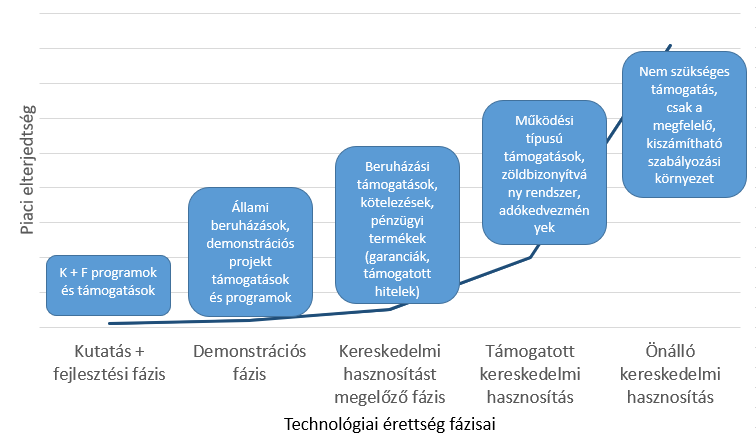
\includegraphics[scale=.7]{support_and_maturity}
    \caption{Technológiai érettség fázisai, és a megfelelő támogatási forma, forrás: saját ábra Foxon et al., 2005 alapján}
    \label{fig:support_and_maturity}
\end{figure}

Ahogy az ábrán is látható, a még kevésbé érett technológiák esetén
(ilyen jelenleg például a széndioxid-megkötés és -tárolás, angolul
carbon capture and storage, vagyis \idxsc{ccs} technológia,
vagy az ár-apály erőművek, 
angolul tide and wave) komolyabb beavatkozás szükséges: konkrét
demonstrációs alapok üzemeltetése, vagy egy-egy projekt állami tőkéből
történő megvalósítása. Kiváló példa erre a 2021 februárjában
bejelentett innovációs verseny is, ahol Elon Musk
100 millió dollár nagyságrendű nyereményt
ajánlott fel új \idxsc{ccs} technológiák kifejlesztésére.

Ilyen projektekre azért van szükség, hogy az elméletből
a gyakorlatba való átültetés során fellépő esetleges problémákat
valós környezetben lehessen tesztelni, egy-egy prototípus segítségével.
Az érettebb technológiák esetén szokásos a beruházási támogatások nyújtása
(sok országban jellemző támogatási forma ez a megújuló hőtermelő
beruházások ösztönzésére), illetve a különböző
pénzügyi eszközök (pl. állami garancia), 
nyújtása, vagy kockázatközösségek szervezése
(utóbbi kettő jellemző például a nagy kezdeti
kockázatokkal járó geotermikus beruházások esetén).

A megújuló energia támogatásának lehetséges módjaival,
az egyes országokban alkalmazott különböző formáival
a korábbi években szerzőtársaimmal közösen
több kutatásban is foglalkoztam. Elsősorban 
a megújuló alapú távhőtermelés támogatását,
ösztönzési lehetőségeit vizsgáljuk néhány évvel
ezelőtti cikkeinkben (Mezősi et al., 2016 és
Mezősi et al., 2017b), ahol modellezés segítségével
elemezzük a magyar távhőpiac lehetőségeit.

A legtöbb megújulóáram-termelő technológia
már túl van a kezdeti fázisokon,
és a ,,támogatott kereskedelmi működés'' szakaszában tart.
Manapság már nem csak a szárazföldi,
de úgy tűnik lassanként az ,,offshore''
(vagyis tengeri) szélerőművek is ide tartoznak,
a naperőművek és a biomassza-, biogázerőművek mellett.

Ezeknek a technológiáknak
ugyan még szüksége van a támogatására,
de már elegendő a működési
támogatások nyújtása, ami az előzőekhez
képest kevésbé nyújt pénzügyi biztonságot a befektetőnek,
hiszen csak a projekt élettartamának legvégére történik
meg a teljes megtérülés, és a teljes kezdeti tőkebefektetést
a beruházónak kell eszközölni. A legtöbb megújuló
projekt esetén a költségek legnagyobb része a beruházáskor merül fel,
az üzemeltetés ugyanis nagyon olcsó,
szemben például egy fosszilis erőművel, hiszen az üzemanyag költség nulla
(ez alól kivételt jelentenek a biomassza és biogáz erőművek).

Tehát, ahogy láthattuk a legtöbb esetben a
megújuló erőművek jövedelmezőségét
manapság már működési támogatás
formájában érdemes elősegíteni. Ez valóban Európa
legtöbb országában ennek megfelelően működik.

A működési támogatásnak is
számtalan formája van azonban, melyek némelyike jobban, mások kevésbé
nyújtanak biztonságot a befektetőnek, és helyeznek ezzel párhuzamos terhet
a támogatási kasszára vagy a rendszer üzemeltetőire.
A következőkben röviden összefoglalom a fontosabb működési támogatási formákat,
és bemutatom, hogy mi vezetett ahhoz,
hogy Európa-szerte egyre inkább eltolódjon a hangsúly
a ,,piackonform'' támogatási formák felé.

Az áramtermelés területén több
működési támogatási forma megkülönböztethető,
de mindegyik lényege, hogy a támogatás valamilyen
módon egy egység (1 MWh vagy 1 kWh)
megújuló forrásból előállított áramra vonatkozik.

Az egyik ilyen támogatás az úgynevezett
(zöld)bizonyítványrendszer, melynek keretében
a kibocsátott zöld áram minden egysége után
egy kereskedhető ,,bizonyítvány'' jár.
Ez a rendszer nagyon hasonlít az \idxsc{eu}
szén-dioxid kibocsátási kvóta kereskedelmi rendszeréhez:
míg előbbiben jellemzően a fogyasztók
(vagy az őket ellátó kereskedők)
kötelezettek bizonyos mennyiségű bizonyítvány
beszerzésére, utóbbi esetén a termelők
kénytelenek megvenni a kibocsátási kvótákat,
hogy tevékenységüket végezhessék.
A bizonyítványok és kvóták árát a kereslet és kínálat
határozza meg. Ilyen rendszerrel találkozhatunk
Romániában, illetve korábban
Lengyelországban is, ahol a megújulók mellett
a kapcsolt termelést (egyszerre áramot és hőt 
is előállító erőművek) is támogatta a rendszer (res-legal, 2019).

Egy másik, sokkal népszerűbb támogatási forma,
az úgynevezett \fit (Feed-in Tariff), 
magyarul legjobban kötelező átvételként
fordítható támogatási forma.
Ennek lényege, hogy a beruházó minden
megtermelt egység áramot 
egy előre meghatározott áron tud értékesíteni
-- jellemzően egy kijelölt piaci szereplő
(ez lehet a rendszerirányító, vagy egy mérlegkör felelős)
az, aki kötelezően átveszi a teljes mennyiséget,
függetlenül attól, hogy az adott órában milyen
árakkal szembesülne a termelő a nagykereskedelmi piacon.

A támogatás tehát nem csak abban áll,
hogy az eladott áram ára fix, hanem abban
is, hogy garantáltan átvételre kerül minden
egység áram (akár abban az extrém helyzetben is,
ha negatív árak alakulnak ki egyébként a piacon,
vagyis bizonyos termelők hajlandóak
fizetni azért, hogy átvegyék tőlük az áramot
-- Németországban a megújulók
ugrásszerű térnyerésével egyre gyakrabban
találkozunk hasonló szituációval).

Ez a támogatási forma tehát nem ösztönzi
a termelőket arra, hogy a keresleti és kínálati
viszonyokat figyelembe véve alakítsák a termelésüket:
amikor süt a nap/fúj a szél, ők biztosan termelni fognak.

Különösen érdekes ez például a biomassza erőműveket üzemeltetők
esetén, hiszen ők nincsenek kitéve
az időjárási viszontagságoknak, így egy másfajta
támogatással könnyedén rávehetőek lennének,
hogy a biomasszát akkor tüzeljék el,
amikor a piacnak is legnagyobb szüksége van az áramra.

Egy \fit típusú támogatási rendszer ezt egyáltalán nem ösztönzi.
Nagy előnye is éppen ebből fakad azonban:
a beruházó várható bevételei függetlenek
a piaci áraktól, ezért a projekt jóval kisebb
kockázattal jár, hiszen az egész élettartam
alatt fix cash-flow számolható -- természetesen
csak azokra az órákra, amikor az erőmű termelni fog,
ezzel kapcsolatosan továbbra is megmarad a bizonytalanság,
főleg az időjárásfüggő erőművek esetén
(szélerőművek és naperőművek).

A legtöbb \idxsc{eu}-s tagállamban ezt 
a formát használták a megújuló energia
támogatására sok-sok éven át.
Bizonyos országokban a mai napig széles
körben elérhető támogatási forma
 -- egyes országokban nemcsak áramtermelés,
de megújuló vagy kapcsolt hőtermelés esetén is.

\fit típusú támogatás manapság is elérhető például
Ausztriában, Franiaországban, Portugáliában vagy Szlovákiában
(res-legal, 2019). A legtöbb helyen (pl.: Horvátország,
Csehország, Németország, Görögország,
Lengyelország, Nagy-Britannia)
azonban csak bizonyos kiemelt beruházói kör jogosult rá,
jellemzően a legkisebb,
háztartási méretkategóriába eső erőművek építői (res-legal, 2019).

Az utóbbi években kialakult óvatosság a
támogatási formával szemben nem véletlen:
több ország is nehéz helyzetbe került az
adminisztratív módon, előre meghatározott
\fit szint bevezetése után. Csehország, Szlovákia
és Spanyolország esete is intő például szolgálhat:
mindhárom ország rendkívül kedvező
támogatási rendszert
vezetett be a 2000-es évek végén, így 2009-2011 környékén ugrásszerűen
megnőtt a napelemek
\footnote{szokás rájuk photovolatikus erőműként, vagy \idxsc{PV}-ként hivatkozni}
száma (Diallo et al., 2018).
Ez nemcsak a hirtelen megugró
támogatási igény miatt volt problémás,
de a rendszerbiztonság fenntartása
is komoly kihívást jelentett a hirtelen
megérkező nagy arányú időjárásfüggő kapacitás mellett.

Amellett, hogy a támogatási forma semmilyen
piaci viselkedésre nem ösztönöz, kellő technológiai
fejlettség mellett láthatóan ,,túl nagy biztonságot''
is jelentett a befektetőknek. Az igazi vonzóerő
azonban még ezek mellett is nagy valószínűséggel
a túl magasan meghatározott átvételi ár volt.

A szabályozóhatóságok ugyanis képtelenek voltak időben lereagálni
a támogatások miatt felfutó iparág fejlesztései nyomán végbement
költségcsökkenést, így az egyre olcsóbb és olcsóbb projektek megvalósítása
ugyanazon átvételi ár mellett egyre jövedelmezőbb volt.
Végül több országban is visszamenőleges módosításokra szorultak,
mérsékelték a támogatást, vagy adókat vetettek ki bizonyos támogatotti körre.

A fenti példák hívták életre, illetve tették
népszerűvé a prémium típusú támogatásokat,
melyek alkalmazása mára a legtöbb
támogatási rendszer esetén \idxsc{eu}-s előírássá vált.
Az úgynevezett \fip (vagy Feed-in Premium)
típusú támogatások esetén a beruházó maga kell,
hogy értékesítse az áramot a nagykereskedelmi piacon,
ezen felül azonban támogatásként egy plusz bevételi elemre jogosult, 
minden egység értékesített áram után.

\label{FIP}
Ennek a plusz támogatás elemnek több formája is lehetséges:
az úgynevezett lebegő prémium hasonlít leginkább a \fit típusú
támogatásokhoz, ekkor ugyanis a kapott prémium nagysága változik (,,lebeg''),
annak megfelelően, hogy mekkora a piaci ár, ugyanis a támogatás
meghatározásakor azt a fix árszintet lövik be, amire a beruházó által
eladott áram árát kiegészítik. Tehát, ha például a rögzített támogatási szint
80 €/MWh, a termelő egyik órában 60, másikban 40 €/MWh-s áron
tudott értékesíteni, akkor első esetben még 20 €-t, a második esetben
még 40 €-t kap minden megtermelt egység (megawattóra) áramért.
Összességében tehát minden egység áramért 80 €/MWh jár neki.

Ez nagyon hasonlónak tűnik a \fit típusú támogatáshoz,
egy fontos különbség azonban,
hogy a legtöbb ország nem számol el 
minden egyes órára vonatkozóan a támogatottakkal,
hanem egy adott időszak átlagos árait veszi figyelembe.
Tehát, ha az adott időszakban az átlagárakhoz
képest egy magasabb termeléssel súlyozott
átlagáron tudott értékesíteni valaki, akkor még jobban is járhat, 
mintha \fit-et kapott volna,
ha alacsonyabb áron, akkor azonban rosszabbul jár.

Ez megteremti egyrészt az ösztönzöttséget arra,
hogy a szereplők reagáljanak a piaci folyamatokra,
másrészt azáltal, hogy a termelőknek maguknak 
kell a megtermelt áram eladásáról
gondoskodniuk elősegíti a piacintegrációt, és a kevésbé torzított
piaci működést (a piac például beárazhatja a vélekedését
az erőművek előrejelzéseinek pontosságával
kapcsolatban hosszabb távú termékek esetén).

Ezen támogatástípus esetén további két
fajtát különböztetünk meg:
a támogatás adható oly módon, hogy ha
a rögzített támogatási szintet meghaladják
a piaci árak, akkor egyszerűen a prémium
elem legyen nulla (a német piacon
például ezzel találkozhatunk), de az is egy
lehetőség, hogy ebben az esetben negatív prémium
alakuljon ki, vagyis a piaci ár előre rögzített támogatási szint
feletti részét a szereplőnek a támogatási kasszába vissza kelljen fizetnie.

Előbbi tekinthető a prémium típusú támogatási rendszerek közül
a legkedvezőbbnek, hiszen a \fit-hez hasonló bevételek szinte biztosan
garantáltak, de még ezen felül is lehetséges további bevétel, ha az áramárak
nagyon magas szintre mozdulnának el (a támogatás pedig az előre meghatározott
szintnél magasabb áramárak esetén egyszerűen nulla, kockázat a támogatás
elszaladásában csak akkor várható, ha az áramárak nagyon leesnek).

Ebben az esetben némi önszabályozás is megvalósulhat,
hiszen ha nagyon megéri (például a magas áramárak miatt)
megújuló erőműveket létesíteni, akkor sok ilyen kapacitás épül,
melyek (a nulla határköltség miatt) egy megfelelő mennyiség üzembe lépése
után lenyomják a piaci árakat (ezt a szakirodalomban ,,merit-order-effect''-nek nevezik,
lásd például: Welisch, M., Ortner, A., \& Resch, G. (2016) ).

A még egyértelműbb ösztönzés a piacon való aktív részvételre 
az úgynevezett fix prémium esetén érhető el.
Ebben az esetben a termelő egy rögzített
nagyságú támogatást kap minden megtermelt
egység áramért, pl. 20 €-t, megawattóránként.
Szintén neki kell gondoskodnia az áram értékesítéséről,
de amennyiben 60 €/MWh-ért tudja eladni az áramot,
akkor összesen 80 €-t kap megawattóránként,
ha csak 40 €/MWh-ért, akkor összesen csak 60 €-t.
Ez tehát még direktebb ösztönzést jelent az erőművek
számára, hogy azokban az órákban termeljenek,
amikor a piacnak legnagyobb szüksége van az áramra.

Itt ismét érdemes megjegyezni, hogy azon termelők esetén,
akik közel 0 határköltséggel termelnek,
ez az ösztönzés gyakorlatilag csak a negatív árak
esetén érvényesül, de például egy biomassza
erőmű esetén (különösen akkor, ha az nem képes az év
összes órájában termelni) már komolyabb hatással
lehet a menetrend tervezésre.

További előny, hogy a naperőművek és
szélerőművek esetén egy ilyen típusú
rendszer az energia tárolását is ösztönzi:
kellően nagy napon belüli árkülönbségek
esetén már előfordulhat, hogy megéri eltárolni
a termelt áramot (például egy lítiumos akkumulátor 
segítségével), és csak akkor értékesíteni,
amikor ez jóval magasabb áron lehetséges.

Az Uniós szabályozás a konkrét támogatási formán túl
számos egyéb tényezőt is rögzített, mellyel igyekszik elősegíteni,
hogy megszűnjön a túltámogatás, és minél zavartalanabb legyen
a megújuló termelők integrációja a villamosenergia-rendszerbe.
Az \idxsc{eu}-s előírások további részleteit a következő fejezetben
ismertetem.

\section{Európai Uniós megújuló politika}

Ebben a fejezetben röviden bemutatom az Európai Unió
megújuló energiához kapcsolódó politikáját.
A fontosabb jogszabályok ismertetésén túl igyekszem az
egyes szabályok mögött álló szándékokat is bemutatni,
valamint rávilágítani, hogy miért volt szükség bizonyos
esetekben a korábbi szabályok módosítására, 
és új megkötések, szigorúbb szabályok szerinti
támogatási rendszerek bevezetésére.

Az Európai Unió megújuló energia támogatására irányuló
politikája szorosan kapcsolódik a klímacélokhoz,
a megújuló energia felhasználásának
növelése azonban számos egyéb
pozitív externális hatással is kecsegtet,
a levegő minőség javulásán
keresztül egészen a fosszilis tüzelőanyagok
esetén az import függőség csökkentéséig.

A klímavédelem és a megújulók azonban olyan
szorosan összekapcsolódnak, hogy az energiapiachoz kapcsolódó
\idxsc{eu} által előírt cselekvési tervek elkészítése (korábban:
Megújuló Energia Hasznosítási Cselekvési Terv) most már 
egy egységes tervként kell, hogy
elkészüljön az ország klímastratégiájával.
Az új dokumentum neve Nemzeti
Energia- és Klímaterv (\idxsc{nekt})
(Európai Parlament és a Tanács, 2018).
A tervek első változatának (tervezetének)
benyújtása 2018 végén, 2019 elején
történt, a végleges változatokat 2019
végéig kellett elkészíteniük az egyes tagállamoknak,
figyelembe véve a Bizottság tervezetek
alapján tett javaslatait.

Az \idxsc{eu} minden tagállamától elvárja a megújuló energia
felhasználás növelését, mely elvárást különböző
megújuló energia felhasználási arányszámokra
vonatkozó célok formájában különböző céldátumokkal
meg is fogalmaz. A konkrét célok ismertetése előtt röviden
bemutatom, hogy pontosan mire is
vonatkoznak ezek az arányszámok,
hogyan kell értelmezni őket, és mi az
oka a számítás ilyen módon történő előírásának.

A megújuló arányszámok a teljes energiaszektort lefedik: 
a közlekedést, a hűtés-fűtési szektort és az áramszektort.
Az arányszám meghatározásakor a teljes megújuló alapú
hazai energiatermelést kell viszonyítani az ország
teljes primerenergia felhasználásához. A mutató tehát azt méri,
hogy az ország a teljes energiafelhasználásának hány százalékát
képes maga megújuló energiából előállítani, fedezni.

Ez a számítási mód azt eredményezi, hogy
előfordulhat 100\%-nál magasabb
megújuló arány is, olyan országok esetén,
amik fogyasztásuknál nagyobb mennyiségben
hasznosítanak megújuló energiát,
természetesen ekkor a fennmaradó többletet exportálják.
Ez azonban nem jellemző: a legfrissebb elérhető adat
a 2019-es érték, az \idxsc{eu}28 átlagos megújuló arányszáma
18,9\%. 50\% felett csupán egyetlen tagállam teljesít,
a meglehetősen előnyös adottságokkal rendelkező
Svédország, a teljes megújuló arány náluk 56,4\% (Eurostat, 2021).

Az egyes szektorok esetén külön-külön is meghatározásra kerültek
az arányszámok, vagyis külön közlekedési, hűtés-fűtési
és áramszektorra vonatkozó arányszámokról is beszélhetünk.
Dolgozatom témájából fakadóan természetesen a
továbbiakra vonatkozóan leginkább releváns mutató
az áramszektorra vonatkozó arányszám. Itt az \idxsc{eu}28-as átlag
2019-re 34,2\%, míg a legmagasabb aránnyal
Ausztria rendelkezik (75,1\%), a fent említett Svédország
pedig 71,2\%-kal követi a második helyen.

Néhány Európai Unión kívüli, környező ország esetén már előfordulnak
100\% közeli, vagy akár azt meghaladó értékek is:
Izlandon az elfogyasztott áram 100,6\%-át,
Albániában 88,5\%-át termelik meg megújuló energia források
segítségével (Eurostat, 2021). Utóbbi esetén a magyarázat, hogy
az ország áramtermelésében semmilyen
fosszilis erőmű nem kap szerepet, az import
mellett gyakorlatilag csak vízerőművekre támaszkodik
az albán áramszektor. Az ország árampiacát részletesen elemeztük
szerzőtársaimmal többek között a South East Europe Electricity Roadmap
(\idxsc{seermap}) kutatás keretein belül (Szabó et al., 2017a). 

Norvégia 2019-ben 110,8\%-os arányszámmal
dicsekedhetett, vagyis jelentősen több megújuló alapú áramot állított
elő, mint amennyit elfogyasztott (mindeközben egyébként
az \idxsc{eu} nagy mennyiségben vásárol Norvégiától
földgázt és kőolajat). Magyarország az utolsó
néhány tagállam között foglal helyet
10,0\%-os arányszámával, míg Németország az átlagot
meghaladó 40,8\%-os arányt ért el 2019-ben (Eurostat, 2021).
Az \idxsc{eu}28-ra vonatkozó adatokat \aref{fig:EU_RES_E}.~ábrán
foglalom össze.

\begin{figure}
    \centering
    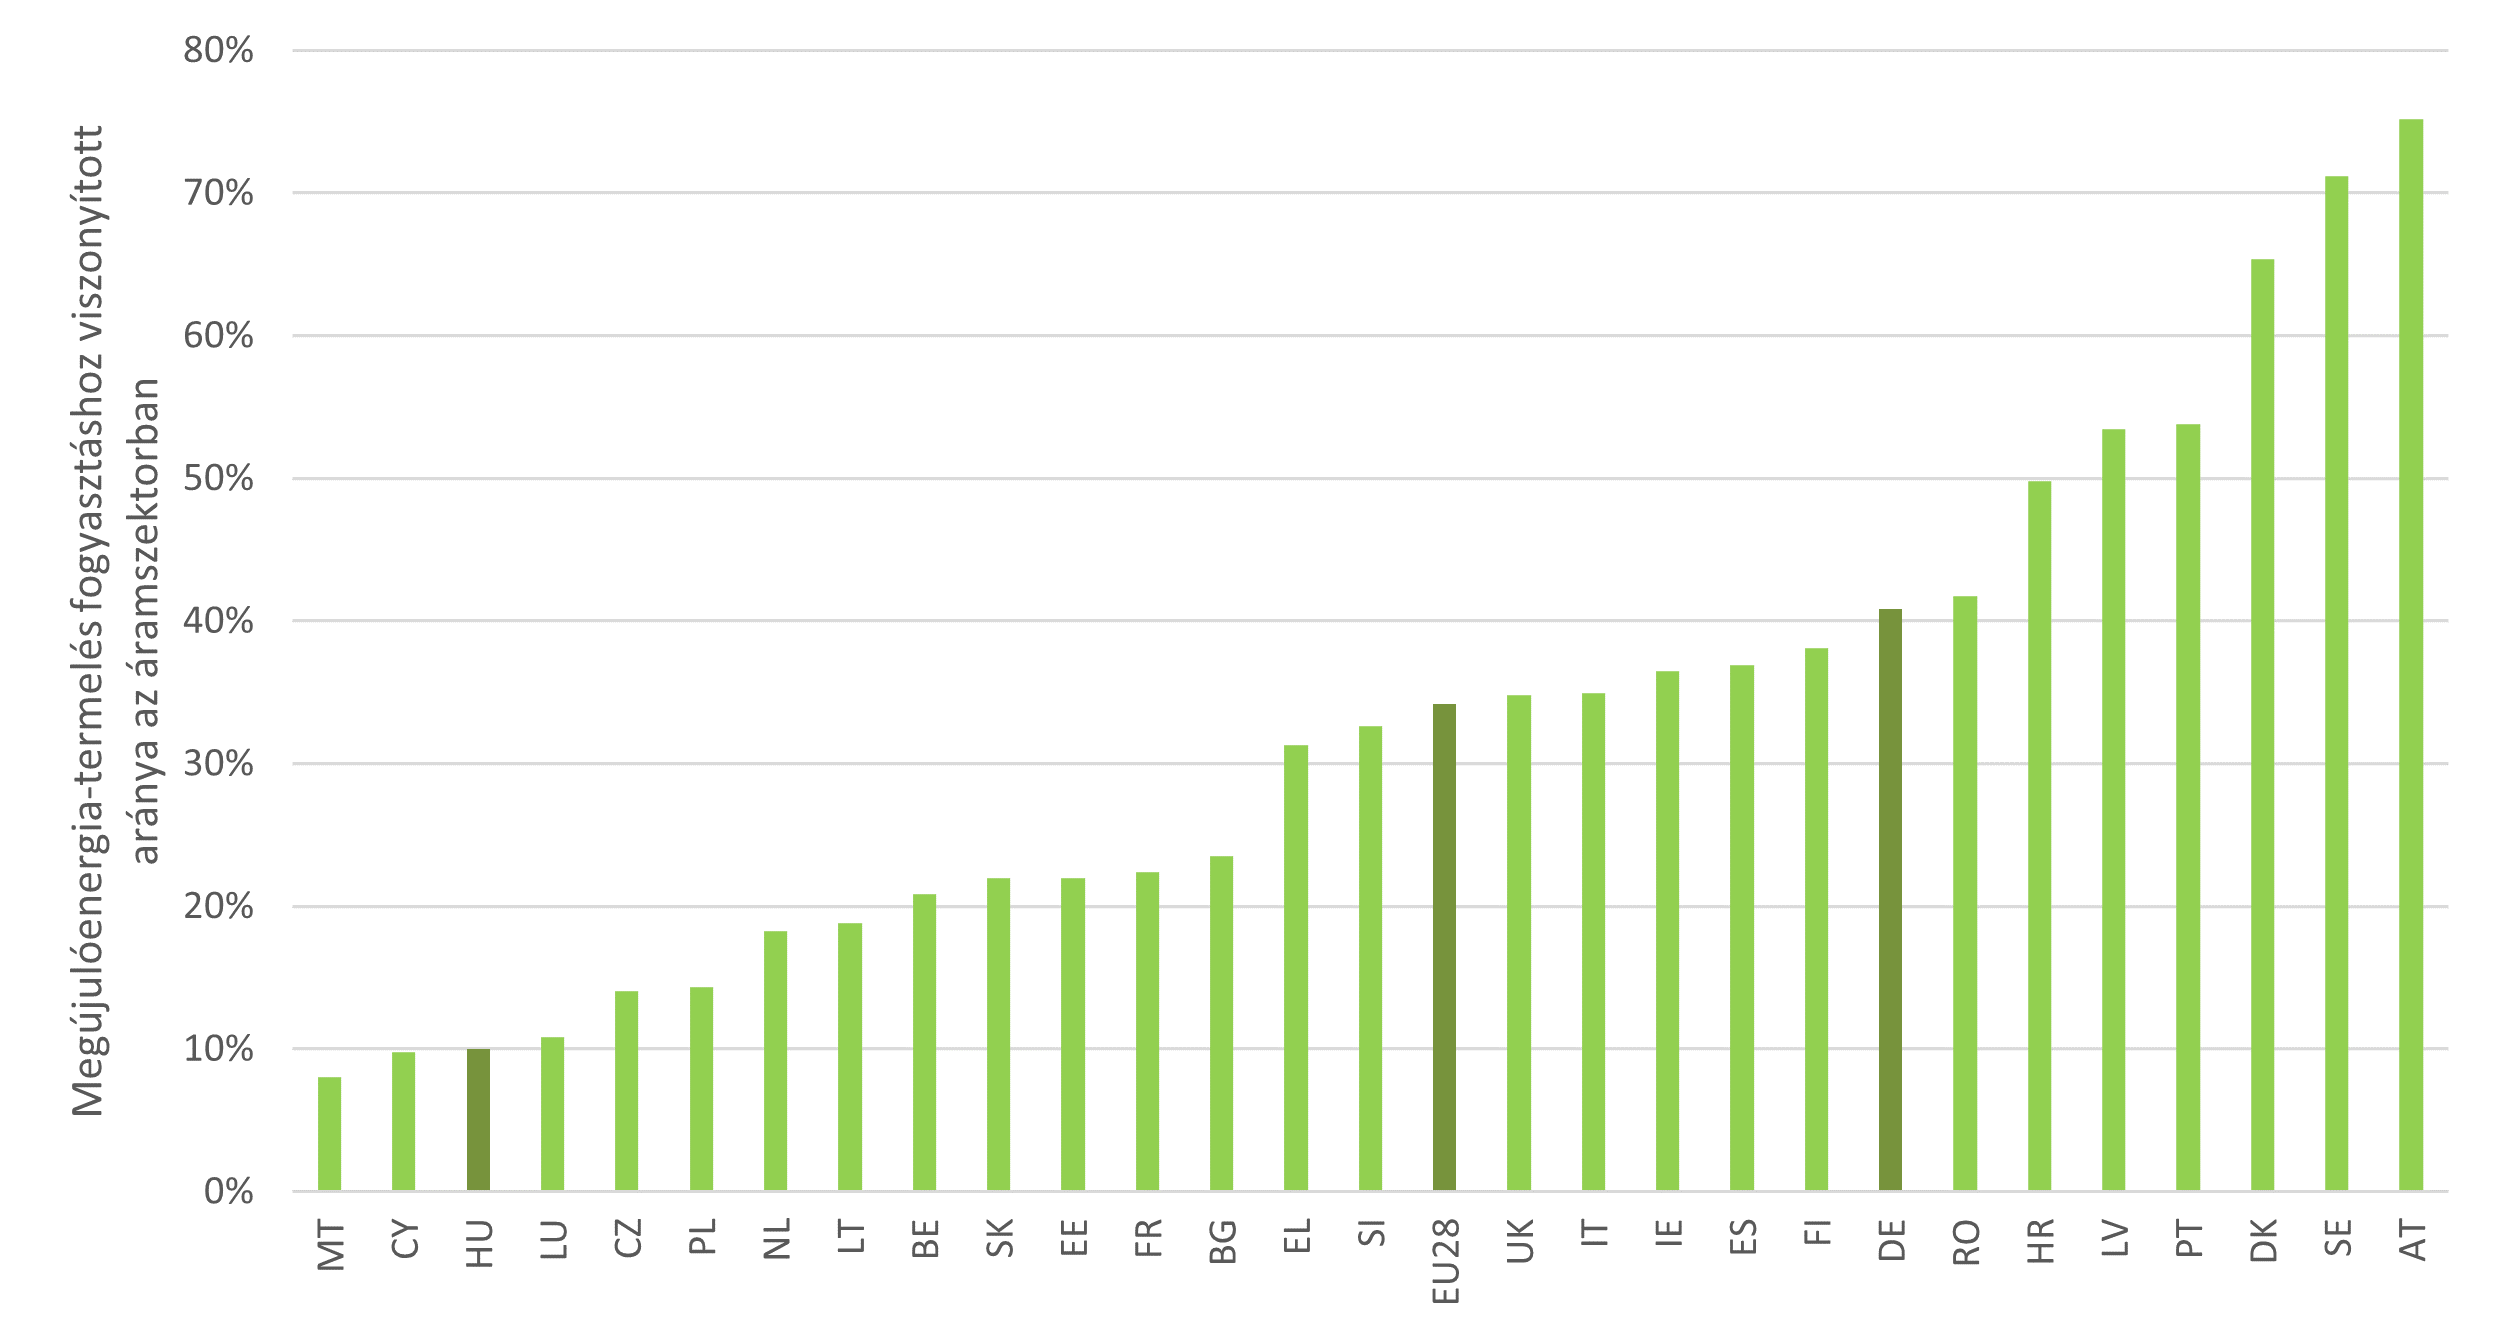
\includegraphics[scale=.65]{EU_RES_E_SHARE}
    \caption{Megújuló energia felhasználási arány az áramszektorban az Európai Unió tagállamaiban, 2017 forrás: Eurostat, 2019}
    \label{fig:EU_RES_E}
\end{figure}

A célok meghatározása 2020-ra (Európai Bizottság, 2009)
és 2030-ra (Európai Tanács, 2014) vonatkozóan különböző módon történt. 
Míg az első esetben a célokat országos szinten fektették le,
addig 2030-ra már Európai Uniós szinten kerültek meghatározásra. 
A 2020-as célok esetén egy össz-\idxsc{eu}-s célt osztottak le az országok
között oly módon, hogy minden ország lehetőségeihez mérten 
kell, hogy hozzájáruljon ezen összesített cél teljesítéséhez.
A megújuló energia mellett két másik fontos célt is kitűztek:

\begin{itemize}
    \item
    20\% üvegházhatású gáz kibocsátáscsökkentés (az 1990-es szinthez képest)
    \item
    20\%-os megújuló energia felhasználási arány
    \item
    20\%-os energiahatékonyság-növelés
\end{itemize}

A leosztás során figyelembe vették többek között
az egy főre eső \idxsc{gdp} értékeket, illetve természetesen azt is, 
hogy milyen kezdőpontból indultak az egyes országok.
Ennek megfelelően a megújuló arány tekintetében viszonylag
széles skálán mozogtak a rögzített értékek: Málta számára 10\%-os
arányt, Svédország számára 49\%-os arányt írtak elő (Európai Bizottság, 2009).

A 2030-as célok ezzel szemben egészen más
logika mentén kerültek meghatározásra.
Az első lépés itt is egy teljes Európai Unióra vonatkozó
cél meghatározása volt, mégpedig a következők szerint:

\begin{itemize}
    \item
    Legalább 40\% üvegházhatású gáz kibocsátáscsökkentés (az 1990-es szinthez képest)\footnote{2020 végén ezt a célszámot az EU 55\%-ra módosította, 2050-re pedig karbonsemlegességet hirdetett. Lásd részletesen: https://ec.europa.eu/clima/policies/eu-climate-action\_en}
    \item
    Legalább 32\%-os megújuló energia felhasználási arány
    \item
    Legalább 32,5\%-os energiahatékonyság-növelés
\end{itemize}

Ezeket a célokat azonban a korábbiakkal
ellentétben nem osztották le országos szintre.
Az \idxsc{eu}-nak együttesen kell teljesítenie ezeket a vállalásokat.
Éppen ezért újra és újra felmerül,
hogy milyen mechanizmust fog választani
az \idxsc{eu} abban az esetben, ha a céldátumhoz közeledve
úgy tűnik nem sikerül teljesíteni a célokat.

Ekkor ugyanis szükség lehet valamilyen
központi beavatkozásra, ami elősegíti, hogy
elérjük a kitűzött csökkentéseket. Az egyik
ötlet ezek közül egy központi aukció szervezése,
melynek költségvetését azok a tagállamok fedezik,
melyek nem haladtak  kellően előre a célok teljesítése terén,
a megújuló energia termelését vállaló
beruházók pedig bármely tagállamból érkezhetnek,
és bármely tagállam területén megvalósíthatják
a projektjüket (Blüchner et al., 2018).
Ez azonban egyelőre nincs napirenden, hiszen egyelőre
a 2020-as célok teljesítésének vizsgálata aktuális.
A célok teljesítését a pandémia miatt visszaeső
kereslet a legtöbb tagállamban segítette.
Kérdés, hogy a gazdaság helyreállása után
az országok képesek lesznek-e a visszazárkózott
kereslet mellett is fenntartani a számokat.

A jogszabályok a 2020-as célok esetén
is lehetőséget biztosítanak arra, hogy egy ország
(részben) egy másik ország területén megtermelt
megújuló energia támogatásán keresztül
teljesítse kötelezettségeit. Ilyen típusú támogatás
kiosztására azonban egyelőre kevés esetben
volt példa -- ezek egyikét, a dán-német közös aukciót
a következő fejezetben mutatom be részletesen.

A 2020-2030-as időszakban azonban
az \idxsc{eu} nemcsak lehetőségként, de bizonyos
országok számára kötelezettségként írta elő,
hogy támogatási rendszerüket kinyissák más országok felé.
Tíz ország (köztük Magyarország) került
a kötelezettek listájára (Blüchner, 2019).

Ennek a szabálynak az oka elsősorban egy versenyhatósági kérdés:
a legtöbb országban a megújuló energia támogatása
a fogyasztóktól beszedett járulékon keresztül történik.
Éppen ezért az import áram -- melyet egy másik
tagállamban termeltek meg -- versenyhátrányba kerülhet az itthon
termelt árammal szemben, ugyanis a járulék rákerül,
a hazai támogatási rendszer juttatásaiból azonban
(az aukció megnyitása nélkül) nem részesülhet.

A jogszabályok másik része a támogatás
kiosztásának módját szabályozta
(Európai Bizottság, 2014). Ahogy fent bemutattam,
több országban is komoly problémákat okozott,
hogy az adminisztratív módon, előre meghatározott támogatás
nem követte le kellőképp a szektorban
időközben bekövetkező költségcsökkenést,
ami annyira kedvező helyzetet teremtett,
hogy egyszerre szinte kezelhetetlen
mennyiségű projekt megvalósulásához vezetett. 

Az \idxsc{eu} ezért bizonyos beépített kapacitás
méret felett betiltotta ezt a fajta támogatást,
és előírta, hogy a támogatási szint
meghatározása verseny keretében történjék.
Az új rendszerben a szereplők aukciókon nyerhetik
el a támogatást, a korábbi automatikus jogosultsággal
szemben, méghozzá oly módon, hogy a támogatás
tényleges szintje is aukción alakul ki, 
és csak egy előre meghatározott keret erejéig
részesülhetnek belőle a jelentkezők.

Egy másik fontos változás -- szintén a nagyobb
méretkategória esetén -- a \fit típusú támogatás
helyett áttérés a \fip, vagyis prémium
típusú támogatásokra. Ahogy fent bemutattam,
ez a támogatási forma sokkal jobban ösztönzi a
termelőket arra, hogy a piaci folyamatokat
lekövetve igyekezzenek előállítani az áramot.

Külön szabályok vonatkoznak a negatív árral
rendelkező órákra: amennyiben az árak 6 egymást
követő órában is negatívak, erre az időszakra
a termelőknek nem adható támogatás. 

A támogatás típusán túl az \idxsc{eu}
előírta a termelők számára a fokozottabb
rendszerintegrációt is. Míg a korábbiakban
a menetrendtől való eltérést a megújulók számára
sokkal kevésbé szigorúan büntették,
az újonnan elnyert támogatások esetén már
maguknak kell fedezni a kiegyenlítési költségeiket,
egy nagyobb pontossággal elvárt menetrendtartás esetén.

A megújuló termelők komoly kihívás elé állították, 
és állítják folyamatosan a villamosenergia-rendszer üzemeltetőit.
Bár az előrejelzések egyre pontosabbak, és a termelők a fenti szabályoknak
megfelelően egyre nagyobb arányban vannak rákényszerítve
a rendszer igényeihez igazított termelésre, a következő évek során
a rendszer fejlesztésére minden tagállamban nagy összegeket kell majd költeni.
A megújulók előretörése ugyanis nem áll meg. A következő
két fejezeteben a német és a magyar árampiac példáján
keresztül szemléltetem ezt.

\section{Támogatások a német árampiacon}

Ebben a fejezetben egy rövid áttekintést adok
a német árampiacról, illetve arról, hogy az utóbbi 
években hogyan alakult a német állam megújuló
energiára vonatkozó politikája,
a közismert nevén ,,Energiewende'', vagyis energiafordulat.
Ennek jelentősége világszerte elismert, nagyban
hozzájárult ahhoz, hogy a megújuló energiához
kapcsolódó technológiák fejlődése megindulhasson.

Ezt követően részletesen bemutatom a jelenleg
érvényben lévő támogatási rendszert,
elsősorban a naperőművek támogatására fókuszálva.
Ez lesz az aukciós modellem kiinduló pontja,
ezért fontos megérteni a működését.

Rövid kitérő erejéig megemlítem a nemrég megtartott
dán-német határon átívelő aukciót, és ennek eredményeit,
mely érdekes tanulságokkal szolgálhat
a megújuló aukciók tekintetében. Különösen
fontos lehet Magyarország számára, 
ahol előírás, hogy a jövőben legalább 
az aukciók egy részét nyissa meg a más
országokban történő beruházások számára is.

\subsection{A német árampiac és az ,,Energiewende''}

A német energiafordulat, vagy közkeletű nevén az ,,Energiewende''
több különböző cél együttes megnevezése.
Röviden összefoglalva olyan limitált szén-dioxid kibocsátású
energiaszektor elérése a cél, melyben a nukleáris energia nem kap szerepet.
A megújuló energia támogatása mellett tehát hosszú távon
a nukleáris erőművek és a szén-alapú termelés teljes visszaszorítása a cél.
Mindezt a versenyképesség szem előtt tartásával, és sok esetben
a lakosság aktív részvételével próbálja meg Németország véghezvinni.

Az Energiafordulat bizonyos tekintetben
már jóval a 2000-es évek előtt elkezdődött.
A fontosabb mérföldkövekről kiváló összefoglalást nyújt
Wettengel (2017), ebből az írásból kiindulva mutatom be én is a fontosabb
állomásokat és döntéseket, amik alapján Németország energiapiaca
elnyerte mai formáját.

Az Energiewende kifejezést az 1980-as évek elejétől
kezdve kezdték el használni,
ekkor alakult meg a Zöld Párt, mely követelte
a nukleáris erőművek bezárását.
Az első két erőművet a két Németország
egyesítésekor zárták be,
ezután még sokáig várni kellett a következő
komolyabb atomerőműveket érintő lépésig.
Mindeközben azonban elindult a megújulókat támogató program:
1991-től kezdődően \fit típusú támogatással igyekeztek
beindítani a megújulók elterjedését.

A 2000-es évben fogadták el -- a később sok
módosítással, de mai napig érvényben lévő -- 
megújuló energia törvényt (Erneuerbare Energien Gesetz -- \idxsc{eeg}).
A törvényben egy \fit típusú támogatás részletei
szerepeltek, 20 éves garantált támogatási
időtartammal, és kötelező átvétellel.
Ugyanebben az évben megegyezést jelentettek
be az áramszolgáltatók és a kormány között
a nukleáris erőművek 2022-ig történő bezárásáról.
Tíz évvel később ismét arról szóltak a hírek,
hogy meghosszabbítják több erőmű élettartamát
is, de csupán, hogy  egy évvel később (2011-ben)
ismét bejelentsék a 2022-es bezárásról szóló terveket.

Az \idxsc{eeg} keretein belül pedig
mindeközben folyamatosan helyezték ki a támogatásokat,
ami a 2002-es 18,5 GW-os összes megújuló
kapacitást tíz éven belül megnégyszerezte
(Fraunhofer, 2019).
2014-ben komolyabb felülvizsgálat történt a rendszerben -- 
eddigre lecsengett több országban is a
fent bemutatott ,,\idxsc{pv}-boom'', tehát Németország
tanulhatott a többiek hibáiból -,
jelentősen lecsökkentették a támogatási szintet,
és a korábbi adminisztratív kiosztás felől 
az aukció irányába mozdultak el.

Az elemzések a 2010-es évek közepétől
kezdődően azonban aggasztóak, úgy tűnik
Németország mindezek ellenére nem éri el
a 2020-ra kitűzött klímacélokat. 
Mi az, amit ennek ellenére elért a német energiafordulat? 
A fenti történet mintegy számszerűsításeként \aref{fig:DE_cap_mix}.~ábrán
a német árampiac termelőinek tíz évvel korábbi,
és a jelenlegi kapacitásait mutatom be a
2019-re elérhető adatok alapján. Jól látható a megújulók
felfutása, és a fosszilis és nukleáris erőművek fokozatos kivezetése.

\begin{figure}
    \centering
    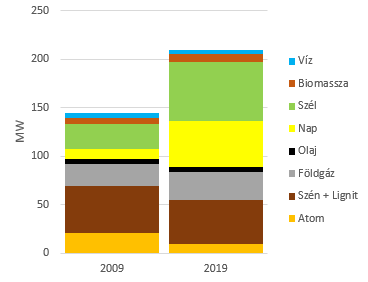
\includegraphics[scale=1.1]{DE_cap_mix}
    \caption{Német kapacitásmix 2009-ben és 2019-ben, forrás: Fraunhofer, 2019}
    \label{fig:DE_cap_mix}
\end{figure}

A rendkívül nagy mennyiségű megújuló
kapacitás telepítése mellett nagyon sok tapasztalat
halmozódott fel, mind a megújuló energiát hasznosító
erőművek gyártása, mind telepítése és üzemeltetése
terén. A komoly támogatás nélkül a szektor
világszerte jóval lassabban érhette volna el a mai költségszinteket,
hiszen éppen a támogatások miatt
volt érdemes a kutatásba, fejlesztésbe fektetni.

Ez meg is hozta a gyümölcsét, hiszen mind a szélenergia,
mind a napenergia esetén drasztikus
beruházási költségcsökkenésnek
lehettünk tanúi az elmúlt 10-15 év során.
2006-ról 2019-re egy friss tanulmány
szerint Németországban összesen 75\%-kal
csökkentek a naperőművi és szélerőművi 
beruházási költségek, ami évről évre több,
mint 10\%-os csökkenést jelent (Wirth, 2019).
\label{invcsokken}

A nagy arányú megújulóval a rendszerben
azonban problémák is jelentkeztek.
A rendszer üzemeltetése komoly kihívást
jelent az időjárásfüggő erőművek esetén,
a rendszerbiztonság fenntartásához a rendszerüzemeltetők
újabb és újabb befektetéseket
kell, hogy eszközöljenek.

Vannak azonban a határokon is átnyúló nehézségek:
Pató (2016) remekül összefoglalja
milyen káros következményekkel kell
a szomszédos országoknak szembenéznie,
ha Németországban hirtelen elkezd fújni a szél. 
A déli országrészben elhelyezkedő atomerőművek
bezárásával az ország korábban kiegyensúlyozottabb
területi ellátása felborult. Míg a fogyasztás komoly
része helyezkedik el itt, az újonnan telepített
szélerőmű kapacitások nagyrészt 
az ország északi részén találhatóak.

Mivel korábban nem volt szükség az országon
keresztül ilyen nagy mennyiségek szállítására,
a belső hálózat nem minden esetben
bírja el a hirtelen jött terhelést, ezért
úgynevezett nem szándékolt áramlások
formájában előfordul, hogy az áram nem
az országon belül jut el északról délre.

A részletekbe való elmélyülés nélkül röviden
(további információért lásd (Pató, 2019)):
a lengyel-német határmetszéken a 2010-es
évek közepén rendkívül sok ilyen nem szándékolt
áramlás történt, az áram ugyanis fizikailag
Lengyelországon keresztül jutott el
Németország egyik pontjából a másikba.
Ez azt jelentette, hogy a rendelkezésre álló
kapacitásokat kereskedelmi célokra nem lehetett
használni, ami komoly veszteséget okozott a lengyel
rendszerirányítónak (panaszát 2015 az
ACER \footnote{Agency for the Cooperation of Energy Regulators,
magyarul az Energiaszabályozók Együttműködési Ügynöksége
-- az Európai Unió által létrehozott szervezet, mely
az energiaszabályozó hatóságok munkáját felügyeli és segíti}
is jogosnak ítélte meg).
Összességében tehát jól látható,
hogy a megújulók elterjedése számos nehézséget
vet fel, de az évek során, ahogy a
tapasztalat is nő, ezek kezelése is egyre könnyebbé válik.

A német átalakulás eddig az áramszektorra fókuszált,
de az utóbbi években egyre nagyobb hangsúlyt
fektetnek más szektorok bevonására: mind a közlekedés,
mind a hőszektor esetén komoly
átalakításokat terveznek.
Ez az autóiparnak is igazi kihívást jelent,
ami a német gazdaság egészét érzékenyen érintheti.
A versenyképesség megőrzése érdekében
az ipari fogyasztók a kezdetektől fogva
mentesültek az egyébként az áramárakba
épített megújuló támogatási elem megfizetése alól.

Az elsősorban a lakosság által megfizetett támogatások hosszútávon,
kellően magas megújuló penetráció esetén elősegíthetik
az áramárak csökkenését (bár a növekvő szén-dioxid-kvótaárak mellett
inkább a növekedés lassításáról érdemes beszélni),
mely maguk és az ipar számára is előnyös lehet,
a közlekedési szektor dekarbonizációjából
fakadó nehézségek azonban már nem oldhatóak
meg a pénzügyi terhek egyszerű áthárításával.

\subsection{A mai német támogatási rendszer}

A támogatási rendszer történetének és
a megújulók elterjedésének bemutatása
után rátérek a ma működő rendszer
szabályainak ismertetésére. Ahogy korábban említettem,
az \idxsc{eeg} szabályozza (Bundesministerium der Justiz und für Verbraucherschutz (2019))
a megújuló energia támogatását, a következő
fejezetben részben erre a jogszabályra, részben pedig Sternkopf (2019)
összefoglalójára támaszkodom.

Ahogy fent bemutattam, Németországban
az aukciók bevezetéséről még 2014-ben döntöttek,
de egy abban az évben megrendezett pilot tender
után az aukciók 2015-től indultak el,
és azóta is folyamatosan tartanak. A részletek
ismertetése a továbbiakban a napenergia
aukciók szabályaira korlátozódik.

Ennek fontosabb ismérvei a következők:

\begin{itemize}

\item
A napelemek esetén (a többi erőműtípushoz hasonlóan) technológiaspecifikus
tendereket rendeznek, vagyis egy-egy aukción csak azonos tüzelőanyagot
hasznosító erőművek indulhatnak. \footnote{Speciális kombinált nap- és szélenergiára
vonatkozó tendereket is szerveznek, de ezek elemzése nem képezi jelen dolgozat tárgyát.}
\item
A támogatás lebegű prémium típusú, 
a szereplőknek arra az árra kell tehát ajánlatot adniuk, amire támogatásként
az állam kiegészíti az értékesítési árukat (a továbbiakban erre az értékre
,,támogatási szint''-ként hivatkozom)
\item
A támogatás 20 évre szól. 
\item
A megvalósítható projektek nagysága 0,75 MW és (földön álló egységek esetén) 10 MW között mozoghat.
\item
Ajánlati biztosítékként
50 €/kW összeget kell rendelkezésre bocsátaniuk az indulóknak
\item
Egykörös, zárt borítékolású aukciókat szerveznek, jellemzően ajánlati áras szabállyal,
de kísérleti jelleggel tartottak egyenáras aukciót is.
\item
Az árplafont havonta módosítják egy előre meghatározott módszertan segítségével.
\item
Évente 3, egyenként 200 MW-os tendert rendeznek, februárban, júniusban és októberben.
A pontos aukcionált mennyiségek azonban egy előre meghatározott módszertan
szerint módosításra kerülhetnek, a már beépült kapacitások mennyiségét figyelembe véve.
\item
A projekt megvalósítására 2 év áll rendelkezésre.
\item
az \idxsc{EU}-s szabályoknak megfelelően amennyiben az árak
6 egymást követő órában is negatívak, erre az időszakra
a termelőknek nem adható támogatás.
\end{itemize}

A támogatási rendszer fenti elemeit igyekszem
a lehetőségekhez mérten részletesen figyelembe venni
a modelleim felépítésekor: mind a pontos költségbecslés,
mind az aukcióelméleti modell esetén.

Néhány elemtől azonban eltekintek. Ezek közül az egyik
az ajánlati biztosíték: ez egy olyan elem, amit
a szereplőknek ahhoz kell befizetniük,
hogy ajánlatot tehessenek. Lényege, hogy
az aukción már csak a ,,komoly'' versenyzők induljanak,
legyen költsége az aukción való részvételnek, hogy
a támogatást elnyerők olyanok legyenek,
akik valóban megvalósítják majd a projektjüket.
Bár ennek a valóságban komoly jelentősége lehet, a modell egyszerűsítése
érdekében eltekintek az ajánlati biztosíték beépítésétől.

A negatív árakra vonatkozó kitétel egyszer
sem volt effektív: az általam készített áramárelőrejelzésben
egyszer sem alakultak ki negatív árak,
a legkisebb ár 2,5 €/MWh volt. Ez azzal magyarázható,
hogy az előrejelzésre használt modell
(lásd részletesen a 3.2 fejezetben) éppen a legextrémebb órákat
képes a legkevésbé leképezni, mert -- ahogy látni fogjuk --,
nem 8760, csupán 90 különböző órát modellezek egy évben.

Ez természetesen némi torzítást visz
az aukcióelméleti modellembe is, de a 6 egymást
követő negatív árral rendelkező óra előfordulása továbbra sem
tekinthető gyakori jelenségnek (bár ez kellő
gyorsasággal felfutó megújuló penetráció esetén változhat).

Mielőtt rátérek a költségbecslés és az aukcióelméleti
modell bemutatására a 3. és 4. fejezetben, egy rövid kitekintés 
erejéig bemutatom két korábbi aukció
eredményeit és tanulságait, melyeket mintegy próbaképp tartott
meg Németország, Dániával közösen.

\subsection{A német-dán határkeresztező aukciók tanulságai}

Érdekes fejleményekkel szolgált az első Európai Unióban
szervezett határonátnyúló (cross-border) aukció,
amit Németország és Dánia közösen hozott tető alá.
A fontosabb tanulságokat Blüchner et al. (2019)
tanulmánya alapján foglalom össze.

A tender kiírására 2016 végén került sor.
A felek két aukció megtartásában állapodtak meg: az egyiket a német fél,
a másikat a dán fél szervezte, és mindkét esetben lehetőség volt
a másik országban telepíteni kívánt erőművekkel is pályázni.
A dupla aukció előnye az volt, hogy mindkét fél a maga képére
formálhatta a szabályokat, így egészen különböző módon történt
a kiírás. A német aukció például egyenárasként, míg a dán aukció ajánlati árasként
került meghirdetésre, mások voltak a projekt méretre és a 
maximális elfogadható ajánlatra vonatkozó előírások is.

A két kiírás mellett olyan szabályok is fontos szerephez jutottak,
amik nem az aukcióhoz, hanem az országhoz kötődnek: többek között
a területhasználat (Németországban például szántóföldön nem telepíthető
napelem, míg Dániában nincsen ehhez hasonló korlátozás), vagy
az adózási rendszer. Ezek a paraméterek függetlenül attól, hogy
a szereplők éppen melyik ország által kiírt aukción vesznek részt
az alapján vonatkoztak rájuk, hogy a projektjüket fizikailag hová szeretnék telepíteni.

Az eredmények a Németország által szervezett aukción a következőképpen alakultak:
a beadott csaknem 300 MW-nyi ajánlat nagyjából fele-fele arányban érkezett
Dániából és Németországból. A nyertesek azonban mind dán területen
megépített projektek voltak. Az előzetes megegyezés alapján ugyan
mind az öt nyertes projekt termelése a német megújuló célhoz járul
majd hozzá, összességében mégis csalódással vették tudomásul a szervezők,
hogy egy ,,saját'' projektet sem tudtak díjazni.

Érdekes módon a Dánia által meghirdetett aukción -- bár szintén nyitott
aukcióról volt szó -- egyetlen német területen megépíteni kívánt projekt
sem indult el. Ennek többek között az lehetett az oka, hogy a szokásos
német (saját, zárt) aukció néhány nappal később került megtartásra,
így a német pályázók valószínűleg inkább az ismert, jobban rájuk
szabott hazai aukción indultak el. Így összességében mindkét aukción csak dán
projektek nyertek támogatást. 

Ennek a sokak szerint meglepő eredménynek a hátterében több 
indok együttesen húzódik meg. Egyrészt Dániában korábban nem szerveztek 
nagy számú aukciót, másrészt a dán napelem-támogatási
programot éppen 2016 májusában zárták le -- a dán beruházók
tehát valószínűleg részben éppen azért indultak versenyképes ajánlatokkal,
mert ezen a két aukción kívül bizonytalannak gondolhatták a további,
jövőbeli lehetőségeket, szemben a német beruházókkal, akiknek folyamatosan
támogatási lehetőséget biztosított a hazai rendszer.

A második fontos tényező a napenergia elérhetősége:
a dán és a német adatokat összevetve azt láthatjuk,
hogy átlagosan a dán adottságok kedvezőbbek, ugyanazzal az erőművel
az időjárási adottságok miatt várhatóan több áram termelhető Dániában.
A harmadik különbségeket megmagyarázó elem pedig a már fent is említett
területhasználat lehetett: a német projektek esetén jóval szigorúbb 
megkötésekkel szembesültek a beruházók, mint a Dániában telepítendő napelemek esetén.

Az aukciókat mindkét ország pilotként aposztrofálta, azonban a megegyezéskor
úgy tűnt, a német fél szeretné a tapasztalatokat kamatoztatni a jövőben
esetlegesen megszervezett további kinyitott aukciókra vonatkozóan is
(a dán fél nem jelezte további nyitott aukciók szervezésére vonatkozó szándékát,
már az egyeztetések során sem). Az eredmények azonban úgy tűnt visszavetették
a németek lelkesedését, így a közeljövőben várhatóan inkább a hazai projektek
támogatására kiírt aukciókra koncentrálnak majd.

A német-dán tenderek tanulsága, hogy fontos látni,
milyen sok különböző tényezőt érdemes figyelembe
venni egy aukció tervezésénél, hiszen mindezek hatással lesznek a szereplők
viselkedésére, és az eredményekre. Ebből a sok tényezőből az egyik kiemelten fontos
a pontos szabályrendszer, ami szerint a szereplők ajánlatait elbírálják, és 
az elnyert támogatási szintet meghatározzák.

Hasonlóan lényeges lehet az is, hogy az aukció kiírója
tisztában legyen a szereplők várható költségszerkezetével,
(ideértve a projektek megvalósításához kapcsolódó adminisztratív terheket is)
és termelési potenciáljával, hiszen így tud egy legalább közelítő képet kialakítani
a várható eredményekről. Dolgozatomban ezért szentelek egy külön
fejezetet a szereplők költségei részletes kiszámításának, ahelyett, hogy
a szakirodalomban fellelhető kész számításokat használnám fel.

\section{Támogatások Magyarországon}

\subsection{A magyar árampiac rövid ismertetése}

A megújuló energia támogatása -- ahogy a következő
alfejezeteben részletesen is bemutatom -- már nagyjából a piacnyitás óta,
tehát, több mint tizenöt éve elkezdődött Magyarországon.
Ennek ellenére igazi áttörés, a megújuló kapacitások
komolyabb elterjedése egészen néhány évvel ezelőttig 
nem történt meg. Az elmúlt egy-két év fejleménye
csupán, hogy egyre több napelem került be a rendszerbe,
és ez a trend várhatóan a következő években is folytatódni fog.

A magyar rendszer azonban még így is meglehetősen
kis részét termeli meg az áramnak megújuló energiából.
A magyar rendszer sajátossága az európai szinten is
magasnak mondható importarány (a 2015-2018-as
időszakban átlagosan 30-35\%), 
valamint a teljes beépített kapacitás 25\%-át adó
Paksi Atomerőmű (Kácsor et al., 2019).

Ahogy \aref{fig:HU_cap_mix}.~ábrán is látható, 
a fosszilis erőműveknek is fontos szerep jut, 
összesen csaknem 4800 MW kapacitás használ
lignitet, földgázt vagy olajat az áramtermelésre.
Több európai országgal egyetemben azonban
Magyarország is bejelentette (a 2019. szeptemberi, new yorki
ENSZ klímacsúcstalálkozón), hogy ,,2030-ig befejezi
a szén energetikai hasznosítását'' , vagyis, szinte biztosan
kikerül majd a Mátrai Erőmű csaknem 900 MW-nyi lignites kapacitása
a magyar mixből (Köztársasági Elnöki Hivatal, 2019).

\begin{figure}
    \centering
    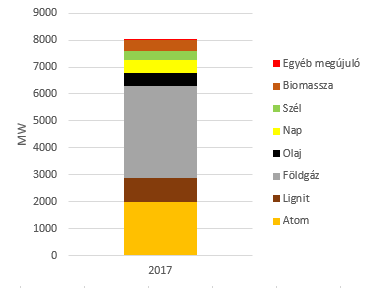
\includegraphics[scale=1.2]{HU_cap_mix}
    \caption{Magyar kapacitásmix 2017-ben, forrás: Mezősi et al., 2019}
    \label{fig:HU_cap_mix}
\end{figure}

A magyar megújuló energia részarány 2017-ben meghaladta a 13,5\%-ot,
(Eurostat, 2019), mely a kitűzött, kötelezően teljesítendő 2020-as cél
(bár az önkéntes vállalás ennél valamivel magasabb, 14,65\%, ezt
azonban nem kötelező teljesíteni 2020-ra, (Bartek-Lesi et al., 2019)).

Ez elsősorban a hőszektorban 
elért magas megújuló penetrációnak köszönhető, ahol 19,6\%-os
megújuló arányt tudott Magyarország felmutatni, hiszen az
áramszektorban csupán 7,5\%, a közlekedésben pedig 6,8\% volt
a megújuló arány 2017-ben (Eurostat, 2019). 
A magyar helyzet speciális, ugyanis az \idxsc{eu} átlagosan jóval nagyobb arányban
teljesít jól az áramszektorban: a fenti arányok a hő-, áram- 
és közlekedési szektorban az \idxsc{eu}28 átlagában 
ugyanerre az évre 19,5\%,
30,7\% és 7,4\%, ami összességében 17,5\%-os teljes
megújuló arányt jelent.

Sajnos a 2018-as és 2019-es évre azonban az arány lecsökkent
(Eurostat, 2021), semmiképpen sem érdemes tehát hátradőlni.
Ennek oka, hogy a hőszektor előretörése a háztartási biomassza
felhasználás növekedésén keresztül valósult meg,
ami részben a korábban magas gázáraknak volt köszönhető.

A hirtelen megugró tüzifafelhasználás részben viszont
statisztikai jellegű: több európai országhoz hasonlóan
Magyarország is változtatott a háztartási tüzifa felhasználás
számítási módszertanán, a korábbi, főként erdészeti statisztikákon
alapuló adatok helyett az új számítás egy a többek között a háztartási
energiafelhasználást is felmérő adatfelvételen alapszik 
(további részletekért lásd: Mezősi et al., 2017).

A rezsicsökkentés hatására, illetve a dráguló tüzifa miatt
azonban sokan visszaváltottak a földgáztüzelésre, így a magasabb 
megújuló arány nem feltétlenül lesz tartható a következő néhány évben.
A pontos arányt ráadásul a hőmérséklet is nagyban befolyásolja, 
ami további bizonytalanságot visz a megújuló célok teljesítésébe.
Éppen ezért kiemelt fontossággal bírnak a hazai
árampiaci tenderek, hiszen a megújuló áramtermelő
kapacitások kiépítése hosszabb távon is biztos megújuló forrásnak
tekinthető, és nemcsak a 2020-as, de a 2030-as célok
teljesítéséhez is biztosan szükségünk lesz rájuk.

\subsection{Történeti áttekintés}

Hazánkban évek óta napirenden van a megújulóenergia-termelés 
támogatásának megreformálása, melyet a fent bemutatott \idxsc{eu}-s előírások
még inkább sürgetővé tettek az elmúlt időszakban.
A korábbi áramtermelésre vonatkozó támogatási rendszer,
az úgynevezett KÁT rendszer (kötelező átvételi rendszer)
még 2003-ban indult, (GKM, 2002; Bartek-Lesi et al., 2019), 
majd később többször módosult (pl. Kormány, 2007), de az
alavető szabályok szintjén egészen 2016-ig nem történt jelentős változás.

A rendeletekben foglaltaknak megfelelően egy \fit típusú támogatást
kaphattak a megújuló energiaforrásból áramot termelők, vagyis minden egység megtermelt
áramért egy előre meghatározott árat kaptak.
A 2000-es évek közepén még mindannyian az úgynevezett
kötelező átvételi mérlegkörhöz csatlakoztak,
nem volt feladatuk a menetrendtartás, amikor termeltek,
a teljes mennyiséget átvette tőlük a mérlegkörfelelős,
egy előre meghatározott áron. 

A fontosabb változások egyike volt, hogy a támogatottak köre bővült:
a kapcsoltan áramot és hőt termelőkre egyaránt vonatkoztak
a fenti szabályok, először csak bizonyos méret alatt,
később pedig egyre szélesebb körben.
Ez a támogatási forma azonban a támogatási igény
jelentős növekedéséből kifolyólag 2010-ben megszűnt
(részletekért lásd: Kácsor et al., 2019).

A \fit típusú támogatások, ahogy fent bemutattam,
ebben az időszakban Európa-szerte
népszerűek voltak, ekkor még a megújuló
energiát hasznosító technológiák költségei
nagyon magasan voltak, így indokolt volt
egy ilyen típusú, rendkívül kedvező, kiszámítható
támogatási forma alkalmazása. Később azonban egyre több
ország példájából vált világossá, hogy 
a támogatási szint meghatározása egyre nehezebb feladat.
Az adminisztratív módon, előre meghatározott
támogatás, illetve a fix áron történő
kötelező átvétel helyett egyéb alternatívákat
kezdtek keresni a döntéshozók.

Az úgynevezett \idxsc{metár} rendszer előkészítése
itthon 2011-ben kezdődött meg.
Az akkor még ,,A megújuló és alternatív
energiaforrásokból előállított hő- és villamosenergia-átvételi
támogatási rendszer'' néven futó törvénytervezet első változata
2012-ben készült el, ebben 2013-as bevezetést
terveztek, erre azonban később mégsem került sor.

A törvényt hosszabb időre félretették,
hogy végül 2016-ban egy olyan változattal álljanak elő,
melyben már az aukción történő kiosztás
és egy prémium rendszer szerepelt, szemben a 2011-2012
során elkészült tervezettel, amiben még fix áron történő
kötelező átvételről írtak.

Már az új \idxsc{metár}-ról szóló rendeletek
címéből is látható volt a változás:
,,a megújuló energiaforrásból származó
villamos energia termelési támogatás
korlátairól és a prémium típusú támogatásra
irányuló pályázati eljárásról'' szóló 
62/2016 \idxsc{nfm} rendelet (\idxsc{nfm}, 2016)
már konkrét aukciós szabályokat tartalmazott.

A teljes támogatási rendszert azonban,
annak minden elemével, részletével együtt
szükséges volt egyeztetni, illetve elfogadtatni
az Európai Unióval, így az aukció tényleges
kiírására még csaknem három évet kellett várni.

Az \idxsc{eu} jóváhagyása után a hazai
piaci szereplőkkel is hosszas egyeztetés
történt, végül az első, ,,pilot'' aukció kiírása
2019 szeptemberében történt meg.
Az ajánlatok beadására októbertől
decemberig volt lehetőség, a
végleges eredményeket pedig a következő negyedévben
hirdették ki. A második magyar aukciót
2020 nyarán rendezték meg, 
az előzetes eredményeket pedig
ősszel tették közzé. A végleges
eredményhirdetés 2021 elejére várható.

A fejezet megírásakor tehát ezek az
eredmények még nem álltak rendelkezésre,
így a fejezet a történei áttekintésen túl a
szabályrendszer részletes bemutatására korlátozódik.
A fejezet legvégén röviden kitérek a két aukció 
(előzetes) eredményeire is.

A szabályok ismertetése előtt azonban
egy rövid kitérő erejéig szeretném bemutatni
a szélerőművi beruházásokhoz kapcsolódó
nehézségeket az elmúlt tíz év során. Bár szorosan
nem kapcsolódik dolgozatom témájához,
úgy gondolom a megújuló energia támogatásának
hazai történetében fontos szerepet
játszik, így érdemel néhány szót.

A szélenergia támogatása -- véleményem szerint
sajnálatos módon -- Magyarországon jelenleg
nem lehetséges, ugyanis 2016-ban egy
miniszteri rendeletben gyakorlatilag
betiltották Magyarország területén a szélerőművek
telepítését (Nemzetgazdasági Miniszter, 2016).

A szélerőművi projektek megvalósítása
azonban korábban sem volt egyszerű
feladat hazánkban. Már az első szélerőművek telepítésekor
-- a rendszerbiztonságra való tekintettel -- 
korlátot vezettek be a kapacitásokra vonatkozóan.
A 2006-ban rendezett tenderen összesen 330 MW
kapacitást engedtek be a rendszerbe, ezek nagyjából öt éven 
belül meg is épültek, és azóta is zavartalanul üzemelnek. 

Több befektető azonban nem fért bele
a megszabott korlátba, így azt várták,
hogy néhány éven belül újabb tenderre
számíthatnak, ahová beadhatják a már előkészített projektjeiket.
2010-ben úgy tűnt meg is érkezik a lehetőség,
a tendert azonban érvénytelenítették.

Többen jelezték, hogy az évek óta húzódó
projekteket (a bennük álló pénz miatt) már támogatás
nélkül is hajlandóak lennének megépíteni, a szabályozó hatóságnak
azonban nem állt módjában tender nélkül
engedélyeket adni, így a beruházók
kénytelenek voltak tovább várakozni.

2016-ban újabb fordulatot vett a szabályozás:
egy miniszteri rendelet (Nemzetgazdasági Miniszter, 2016)
de facto megtiltotta a Magyarország területén történő szélerőmű létesítést,
amikor a szabályokat a következőképpen módosította:

\textit{,,Beépítésre szánt területen
és beépítésre szánt terület határától számított 12 000 méteren belül –
a háztartási méretű kiserőműnek számító szélerőmű kivételével –
szélerőmű, szélerőmű park nem helyezhető el.'}' (Nemzetgazdasági Miniszter, 2016)

Ezzel az egyetlen módosítással teljes Magyarország területén került
megtiltásra a szélerőművek létesítése, ugyanis a 12 km-es 
védőtávolság olyan szigorú, hogy az ország egyetlen pontja sem felel
meg az újonnan előírt kritériumnak (Kotek, 2016).
Ahogy látni fogjuk, a magyar aukció várható eredményeire
ez a körülmény nagy hatással lehet, hiszen egy -- nemzetközi
példák alapján kifejezetten versenyképesnek mondható -- technológiával
kevesebb indul majd a tenderen.

Az aukció résztvevőivel és a finanszírozással kapcsolatban érdemes még egy
körülményt kiemelni. Ahogy fent említettem, az aukció bevezetéséről egy
2016-os jogszabály döntött. Ugyanekkor került
rögzítésre az is, hogy az akkor életben lévő támogatási rendszer
megszűnik (pontosabban átalakul), de az év végéig beadott engedélykérelmek
esetén még az aktuális szabályok érvényesek, csak a 2017. január 1. után
engedélyért folyamodó erőművek lesznek kötelesek az esetleges
támogatás elnyeréséhez aukción elindulni.

Ez a változás valóságos dömpinget indított el: 2016 december végéig
csaknem 2000 MW naperőművi kapacitásra érkezett be
engedélykérelem. Ez, a miheztartásvégett -- bár termelésben közel
sem jelenti ugyanazt -, kapacitásban a Paksi Atomerőműnek felel meg.
A szereplők ugyanis attól féltek, hogy az aukciókon
jóval alacsonyabb támogatási szintek alakulhatnak ki
(ahogy látni fogjuk, nem alaptalanul),
illetve a prémium típusú támogatásra való átállás a kötelező átvétellel
szemben kockázatosabb, és így nehezebben is finanszírozható.

Sokáig kérdés volt, hogy valóban megépül-e mind a 2 GW kapacitás,
de az elmúlt egy-két év során rendkívül nagy mennyiségű
napelem került be a rendszerbe, így várhatóan szinte a teljes
kapacitás megjelenik majd (bár a két év 
már eltelt, még nem áll rendelkezésre minden adat
a kérdés megválaszolásához). Sok potenciális befektető tehát 
már ebben a körben megvalósította a projektjét, ez biztosan
csökkentette a résztvevők számát az aukción. Fontos azonban megjegyezni,
hogy az elmúlt három év során világszerte még tovább csökkentek 
a napelemek beruházási költségei, így előfordulhat, hogy
sokkal több projektet éri meg most megvalósítani, mint 
néhány évvel ezelőtt.

A finanszírozást azonban több piaci szereplő
(köztük a Bankszövetség és a \idxsc{mekh}) szerint is nehezítheti,
hogy a szektorban való kitettség a kötelező átvételre
jogosult erőművek gyors felfutásával, 
és ennek finanszírozásával közel kerülhetett a kritikus szinthez:
a bankok nem feltétlenül lesznek ugyanolyan nyitottak
a projektek hitelezésére, mint voltak a nagy arányú
energiapiacon történő hitelkihelyezések előtt.

További nehézség lehet, 
hogy a bankok számára a támogatási forma  
és a szigorúbb menetrendtartási kötelezettség is újdonság,
ráadásul kockázatosabb is, mint a korábbi kötelező átvételi
rendszer volt. Kérdéses volt tehát, hogy rendelkezésre fog-e állni
kellő forrás a bankszektorból, hogy megfelelő számú
résztvevővel indulhasson el az első magyar aukció.
Ahogy látni fogjuk, úgy tűnik ez végül nem jelentett problémát,
sikerült megugrani az akadályokat.

\subsection{A magyar aukció szabályrendszere és az eddigi aukciók eredményeinek rövid elemzése}

A hazai aukció szabályai a legtöbb európai
tendertől viszonylag sok ponton különböznek.
Az egyik legelső és legfontosabb különbség,
hogy a legtöbb jelenleg is futó rendszerrel ellentétben
a magyar aukció technológiasemleges.

Ez azt jelenti, hogy a különböző technológiát
alkalmazó befektetők egymással versenyeznek:
vagyis a naperőművet, biomassza tüzelésű erőművet,
geotermikus erőművet megvalósítani kívánó befektetők egyszerre adnak
ajánlatot, és a legalacsonyabb támogatást
kérő befektetők nyernek, függetlenül attól,
hogy mely technológiával szeretnének megújuló energiát termelni.

Ahogy fent láthattuk, a szélenergia
nem vesz részt a versenyben. Amennyiben a későbbiekben
a 2016-os szabályok eltörlésre, vagy enyhítésre
kerülnének, a jelenlegi kiírás alapján már
részt vehetnének a szélerőművek is az aukción,
jelenleg ennek egyetlen akadálya a 2016-os miniszteri módosítás.

Itt rögtön szeretnék kitérni arra, hogy dolgozatomban miért nem a magyar aukció elemzését
választottam központi témámnak. Az aukcióelméleti keretrendszerben történő
modellezés során komplex optimalizációs feladatokat kell megoldani.
A szimmetrikus aukciók esetén ezek a feladatok jóval kevésbé bonyolultak,
mint az aszimmetrikus esetben, a modelleket könnyebb mind felírni, mind megoldani.

A fent említett technológiák igen különbözőek, mind költségszerkezetüket,
mind üzemeltetési lehetőségeiket tekintve. Bár mindezt egyetlen számba
sűríthetjük az \idxsc{lcoe} számítás során (lásd 3. fejezet), 
de a szereplők közötti különbségek jelentősek maradnak, így az aukciót
aszimmetrikus, legalább három különböző típusú szereplőt feltételező
módon kellene modellezni, ami rendkívül komplex feladat.

A magyar aukció másik érdekessége,
hogy kettős korlát szabja meg a nyertesek számát.
Egyrészt a 2016-os rendeletben szereplő
módon adott egy maximális költségvetés.
A kért támogatások összesítve éves szinten
nem haladhatják meg az 1 milliárd Forintot, 
mely korlát tovább van bontva két méretkategória között:
0,3 MW-nál nagyobb, de 1 MW-nál
kisebb névleges teljesítőképességű erőműegységek
esetén a kiosztható éves támogatásra
vonatkozó korlát 333 millióFt, legalább 1 MW, de legfeljebb 20 MW-os
névleges teljesítőképességű erőműegységek 
esetén pedig 667 millióFt (\idxsc{mekh}, 2019).

Ezen túl a végleges, 2019-es kiírásban már egy
támogatott villamosenergia-mennyiségre vonatkozó korlát
is szerepel: a kisebb méretkategória esetén ez 66 GWh/év,
a nagyobb esetén 134 GWh/év (tehát mind a költségvetés,
mind a támogatandó energiamennyiség 1/3:2/3 arányban oszlik
meg a két méretkategória között, (\idxsc{mekh}, 2019)).

A dupla korlát miatt tehát előfordulhat, hogy kellően kedvező ajánlatok
esetén nem a költségvetési korlát lesz effektív, mert a támogatott energiamennyiség
már meghaladja a mennyiségi korlátot, így az erre szántnál kevesebb
pénzből támogatható a megszabott mennyiségű áram megtermelése.
Erre az utólag bevezetett mennyiségi korlátra (a 2016-os jogszabályban még
nem szerepelt ez a kitétel, csupán a végleges aukciós kiírásban)
a rendszerbiztonság fenntarthatósága miatt volt szükség.

A második, és talán fontosabb oka, hogy nem a magyar aukciókat elemzem
ez a fajta dupla korlát, illetve elsősorban az összköltségre vonatkozó korlát megléte.
Az aukcióelméleti irodalomban sztenderd módon használt
modellek konkrét számú aukciónált termékkel számolnak.

Ahogy később a 4. fejezetben látni fogjuk,
a modell logikája, hogy adott egy bizonyos számú
termék, melyeket eladni, vagy éppen megvenni szeretne az aukció kiírója.
Ehhez ajánlatokat kér be a szereplőktől, majd ezeket sorbarendezi,
és a legjobb ajánlatot adóknak adja oda a (teljesen megegyező) termékeket.

A nyerés valószínűsége az alapján számítható egy adott ajánlat esetén,
hogy ez az ajánlat várhatóan hanyadik lesz a sorban: ha ez a sorszám kisebb,
mint az aukcionált termékek száma, akkor a szereplő az adott ajánlattal nyerni fog,
ha nagyobb, akkor nem nyer. 

Ha azonban a nyertesek pontos száma nem ismert előre, mert előfordulhat, hogy
a költségvetési korlát szabja majd azt meg, a fenti logika nem alkalmazható,
a számolást egész másképp kellene felírni és végrehajtani. 
Ez az aukcióelméleti irodalomban bevett modellek jelentős módosítását igényelné,
a szakirodalomban egyelőre nem találkoztam hasonló modell kidolgozásával,
így magam sem vállalkoztam erre a nehéz feladatra.

A szabályok bemutatása után pedig röviden összefoglalom
az időközben megrendezett két aukció eredményeit.
Ehhez Bartek-Lesi et al. (2019b), Kácsor (2020) és Varga (2020a) és Varga (2020b) 
rövid elemzéseit hívom segítségül.

Ahogy fent említettem, az aukción két méretkategóriában lehetett indulni.
Az első aukción a két méretsáv 0,3-1 MW és 1-20 MW volt,
míg a második aukción ez valamelyest módosult, a nagyobb kategória
felső határa 49,99 MW-ra növekedett. Ezzel párhuzamosan
a teljes támogatott mennyiség is csaknem kétszeresére nőtt, 
66+134 GWh/év-ről 40+350 GWh/év-re
(az első aukciót még pilotként aposztrofálták, a másodikat már nem).

Mindkét aukción alaptalannak bizonyult a félelem a finanszírozás
nehézségeivel kapcsolatban -- legalábbis ezt látszik alátámasztani 
a túljelentkezés nagyságrendje. A támogatható éves termeléshez
képest 1,5-, illetve 2,5-szeres volt a beadott ajánlatokhoz tartozó
termelés mennyiség, vagyis igazi verseny bontakozott ki.
A második aukción -- bár itt az eredmények egyelőre csak előzetesek --
ugyanezen arányszámok nagyjából 4,5 és 5,5-szeresnek adódtak (MEKH, 2020).
A jelentkezők túlnyomó többsége naperőművi projekttel
indult. Az első aukción összesen egy induló volt, aki egyéb
(hulladékhasznosítóból származó gázt hasznosító) erőművel
pályázott, a második aukción már két ilyen és egy geotermikus
erőmű is elindult. Az összes 153, illetve 272 résztvevő közül azonban
elhanyagolható a számuk. 

A verseny megmutatkozott a kialakuló árakban is. Míg a korábbi,
kötelező átvételi ár közel 100 €/MWh volt, addig az aukción
kialakuló súlyozott átlagárak (Ft/kWh-ról 2019 decemberi árfolyamon átváltva)
74,3 és 65,6 €/MWh-nak adódtak a kisebb és nagyobb méretkategóriában
az első aukción. A második aukción még nincs végleges eredmény,
de a beadott ajánlatokat már közzétették, ezek alapján
további jelentős árcsökkenés várható, az ajánlatok ugyanis
25-30\%-os csökkenést vetítenek előre. 

A magyar aukciók tehát egyelőre sikertörténetnek mondhatóak,
bár az erőművek megvalósítási rátáit még nem ismerjük,
erről a következő néhány évben tudunk majd biztosat mondani.
Az eddigi eredmények azonban biztatóak,
és alátámasztják a támogatások aukción történő
kiosztásának költséghatékonyságát.

\chapter{\textsc{lcoe} számítás}

\scwords A szereplők értékelése az aukciós
modellek egyik legfontosabb pontja,
ami a támogatásokra vonatkozó aukciók esetén
a költségeiknek vagy a támogatásigényüknek feleltethető meg.
Egy szimmetrikus aukció esetén minden szereplőnek
ugyanabból az eloszlásból származik az értékelése/költsége,
ez az eloszlás köztudott tudás, az ajánlatadás pillanatában
pedig mindenki csak a saját realizációját ismeri.
A következő fejezetben ennek a
költségeloszlásnak a meghatározását mutatom be.

Először ismertetem az eredeti \idxsc{lcoe} számítás logikáját,
illetve a szakirodalomban fellelhető
adatok alapján a német \idxsc{pv} technológia esetén becslést is készítek.
Ezt követően bemutatom az aukciós
modellemhez használt módosított \idxsc{lcoe} számítást,
és annak eredményeit. 

\section{Fajlagos áramtermelési költség (\textsc{lcoe}) számítás}

Az \idxsc{lcoe} (Levelised Cost of Electricity)
egy villamos energia termelő egység esetén
a fajlagos áramtermelés költségét ragadja meg.
A teljes élettartamot,
és az ez alatt felmerülő minden kiadást figyelembe véve
mondja meg az egységnyi megtermelt áramra eső költséget.

Úgy is tekinthetünk rá, mint az az 1 energiaegységre jutó állandó bevétel,
ami mellett a projekt bevételeinek és kiadásainak jelenértéke éppen megegyezik:
vagyis ekkora energiaegységenkénti
(pl. megawattóránkénti) bevételt kell realizálni ahhoz,
hogy a beruházás az elvárt hozamot is figyelembe véve éppen megtérüljön.

Egy egyszerű \fit rendszer esetén a termelők tehát legalább akkora
(a projekt teljes élettartama alatt) fixen megkapott ár
mellett valósítanák meg a beruházást,
amekkora a projektjükre vonatkozó \idxsc{lcoe} érték.
Ha tehát egy \fit rendszerben vizsgálnánk
a szereplők ajánlatadási viselkedését,
akkor az eredeti keretrendszerben szereplő értékelés
éppen az \idxsc{lcoe} értéknek felelne meg.

A szakirodalomban rendkívül bevett módszer,
hogy az egyes technológiákat
ezen mutató mentén hasonlítják össze egymással.
Ennek megfelelően
viszonylag sok adat áll rendelkezésre mind a tényleges \idxsc{lcoe} értékek becslését,
mind a számításuk során használt inputok becslését tekintve.
A német piacra vonatkozóan ez különösen igaz,
hiszen az elmúlt évek során
a szabályozás elkötelezett módon igyekezett minél nagyobb
mennyiségű megújuló erőmű létesítését elősegíteni,
és -- ahogy ezt a bevezetőben is láthattuk -- ezt sikerrel is tette.

A német példa világszerte ismert és elismert,
ezért a megújuló energiaköltségekkel
foglalkozó tanulmányok a legtöbb esetben külön foglalkoznak vele,
illetve a nagyszámú projekt megvalósítása miatt tényadatok is rendelkezésre állnak.
A magyar piac esetén már sokkal kevésbé érhetőek el országspecifikus adatok,
így ott az \idxsc{lcoe} becslés is bizonytalanabb és nehézkesebb,
ez egy újabb indok volt a német piac vizsgálata mellett.

Az \idxsc{lcoe} számítás levezetését nem
az induló definíció segítségével végzem el,
vagyis nem egyszerűen az egy energiaegységre jutó
költséget írom fel, hanem azt az energiaegységenkénti állandó bevételt
keresem meg, ami mellett a költségek és bevételek nettó jelenértéke
a projekt egész élettartamát tekintve
éppen egyenlő lesz. A számítások során minden 
költséget és bevételt reálértéken veszek figyelembe,
2019-es euróban számolok.

Ehhez tehát első lépésként fel kell írni ezt a két jelenértéket,
majd ebből kifejezhető az \idxsc{lcoe} érték.
A számítás során a következő tételeket szokás figyelembe venni:

\begin{itemize}
    \item
        $I$: Beruházási költség (a nemzetközi szakirodalomban capital cost, vagyis \idxsc{capex})
    \item
   $M_t$: Üzemeltetési és karbantartási költségek (éves szinten) -- a nemzetközi szakirodalomban
operation and maintanance cost (O\&M) vagy operational expenditures (\idxsc{opex})
    \item
    $E_t$: Megtermelt (és hálózatba táplált) villamos energia mennyisége (éves szinten)
    \item
    $r$: Elvárt megtérülés -- a számításaimban a súlyozott átlagos tőkeköltség (a nemzetközi
szakirodalomban Weighted Average Cost of Capital – \idxsc{wacc}) felel meg az elvárt hozamnak,
amennyiben mindent reálértéken veszünk figyelembe
    \item
    $n$: Projekt élettartam
\end{itemize}

Szokás még figyelembe venni az éves tüzelőanyag költséget,
ami sok erőműnél igen jelentős (pl. fosszilis vagy biomassza tüzelés esetén).
A naperőművek esetén azonban ez a költség 0,
így nem kerül bele a számításba.

A számítás tehát a következőképpen történik:

\[
        \sum income = \sum_{t=1}^n\frac{E_t LCOE}{(1+r)^t}
\]

A megtermelt energia mennyiségének és 
az energiaegységenkénti bevételnek a
szorzatát minden időszakban kiszámítjuk,
és ezen összegek nettó jelenértékeként
kapjuk meg a bevételi oldalt.

\[
        \sum cost = I (1+r)^0 + \sum_{t=1}^n\frac{M_t}{(1+r)^t}
\]

A kiadások az időszak első pillanatában felmerülő
\footnote{szokásos feltételezés, hogy a beruházási költségeket
nem a valósághoz közelebb áll módon időben elosztva,
hanem a projekt legelején, egyösszegben vesszük
figyelembe, ez az úgynevezett "overnight investment cost".}
beruházási költségből, és a későbbi időszakok folyamán
fellépő üzemeltetési és karbantartási költségekből állnak össze.

\[
        \sum income = \sum cost
\]

\[
LCOE \sum_{t=1}^n\frac{E_t}{(1+r)^t} =  I (1+r)^0 + \sum_{t=1}^n\frac{M_t}{(1+r)^t}
\]

\[
LCOE = \frac{ I + \sum_{t=1}^n\frac{M_t}{(1+r)^t}}{\sum_{t=1}^n\frac{E_t}{(1+r)^t} }
\]


A jelölések a fentieket követik: $n$ az élettartamot,
$E_t$ a t. évben megtermelt áram mennyiségét,
$r$ a feltételezett (reál) \idxsc{wacc}-ot (vagyis az elvárt hozamot)
$I$ a beruházási költséget, $M_t$ a t. évben fellépő működési költségeket jelöli.

A számítás ezen változata a költségelemekkel kapcsolatban
a következő implicit feltételezéseket tartalmazza:
\begin{itemize}
    \item 
    A beruházást a 0. időpillanatban fizeti ki a szereplő,
egy összegben
    \item
    Minden további költség (és bevétel) az adott időszak elején merül fel (szintén egy összegben)
\end{itemize}

A következőkben röviden összefoglalom a legfontosabb forrásokat,
melyekre a saját \idxsc{lcoe} számításom elkészítésekor támaszkodom.
A szakirodalomban jellemző, hogy a szerzők nagy kutatóintézetek
és nemzetközi szervezetek által rendszeresen közzétett riportok,
és más cikkekben szereplő adatok alapján készítenek
saját számolást (pl. Shrimali et al, 2016; Welisch, 2019),
de előfordul az is, hogy a saját modelljükben
már csak felhasználják ezeket az adatokat
(pl. Viana \& Ramos, 2018; Mezősi et al., 2018).

A német Fraunhofer Institute 2010 óta folyamatosan
készít elemzéseket a megújuló energia költségeihez kapcsolódóan.
Egyik legfrissebb, 2018-as anyaguk (Fraunhofer, 2018)
a német piacra vonatkozóan mutat be becsléseket.
Három \idxsc{pv} méret esetén is számít \idxsc{lcoe}
értékeket (kisebb és nagyobb tetőre szerelhető,
illetve még nagyobb földön álló termelő egységek), 
ezentúl szárazföldi és partmenti szélerőművek, biogáz,
illetve fosszilis erőművek esetén is elvégzik a költségbecslést.

A számításhoz részletesen közzéteszik
az összes bemeneti paramétert és egyéb feltételezést is.
A következő tételekre találhatunk információt
az anyagban, technológiánként: beruházási költség
(\idxsc{capex}), üzemeltetési költség (\idxsc{opex}), 
élettartam, hatékonyságromlás, és minden részlet a \idxsc{wacc}
(weighted average cost of capital, vagyis súlyozott tőkeköltség)
kiszámításához (saját tőke és idegen tőke aránya, 
előbbin elvárt hozam és utóbbi esetén a hitel kamatszintje). 

Szintén a német piacra fókuszál egy 2015-ös
Fraunhofer anyag (Fraunhofer, 2015).
A fentivel ellentétben itt kizárólag a \idxsc{pv} 
rendszerek költségeit elemzik, és a fókusz a 2014-es 
tény értékek bemutatása mellett egy hosszútávú,
2050-re vonatkozó előrejelzés elkészítésén 
van a költségek alakulását illetően.
A beruházási és üzemeltetési költségek,
valamint a kamatláb mellett itt az inverterek
élettartam közepe táján esedékes cseréjéről,
és az ehhez kapcsolódó költségekről is szó esik. 

Lazard (2017) az amerikai piacot vizsgálja,
5 különböző \idxsc{pv} technológia mellett többek
között geotermális erőműveket és üzemanyagcellás megoldásokat is vizsgál,
illetve összeveti ezek múltbeli költségeit a konvencionális áramtermelőkével.
A költségekre vonatkozóan megvizsgálják a különböző támogatások,
a kamatlábak és a tüzelőanyagár-
változások hatását is,
és külön kitérnek az egyes egységek szén-dioxid-kibocsátására is.

Szintén fontos forrás a Nemzetközi Energia
Ügynökség (International Energy Agency -- \idxsc{iea})
két friss anyaga (IEA, 2018 és IEA, 2017).
Előbbiben országokra lebontva kaphatunk képet
az elmúlt évek legfontosabb fejleményeiről a napenergia kapcsán.
A szerzők több Európán kívüli ország esetén is
(pl. Argentína, India, Chile, Szenegál, Brazília) elvégzik a költségbecslést.

Utóbbiban pedig részletesen elemzik a korábbi
aukciókon kialakuló árakat több különböző technológia esetén,
és előrejelzést is készítenek 2022-ig bezárólag.
A napenergia esetén két méretkategóriát 
különböztetnek meg (háztartási és nem háztartási). 

Az \idxsc{iea} korábbi anyagaiban (pl.: IEA, 2015)
szintén fontos adatok vannak összegyűjtve a különböző
megújuló technológiák jelen és jövőben várható költségeit tekintve.
Az országos szintre lebontott adatok között
három különböző méretkategóriát találunk a német napenergia termelőknél,
és az \idxsc{lcoe} értékek különböző kamatszintek 
(\idxsc{wacc} feltételezések) mellett kerülnek kiszámításra. 

Végül megkerülhetetlen forrás az IRENA több kiadványa is
(IRENA, 2016 és IRENA, 2018).
Előbbi annak fontosságát hangsúlyozza, hogy
a növekvő versenyhelyzet és a megfelelő ösztönzők
tovább növelhetik az innovációt a megújuló energia szektorban,
ami folyamatos költségcsökkentést eredményezhet a jövőben.

Utóbbiban az országokra és technológiákra lebontott
költségadatokat nemcsak riport formájában,
de táblázatos adatként (Excel formátumban) is közre adták.
Az adatok segítségével 2009-től 2017-ig
negyedéves bontásban láthatjuk több ország esetén is
a beruházási költségek és az \idxsc{lcoe}
értékek alakulását a különböző országokban,
és rengeteg világszintű összesítő adatot is találunk.

\Aref{tab:forrasok}.~táblázat a fent bemutatott
forrásokban szereplő adatokat,  és az utolsó oszlopban a
saját számításomban figyelembe vett értékeket foglalja össze.

A riportok nagy részében külön méretkategóriákra bontva szerepeltek értékek. 
Jellemzően lakossági és e fölötti bontást találunk
(angolul tipikusan: „residential” vagy „rooftop”,
illetve „utility scale” megnevezéssel). 
Mivel az aukció potenciális résztvevőinek
költségeit igyekszem számszerűsíteni, ezért a „utility scale”
méretkategória számait gyűjtöttem össze.

\label{invcost}

\begin{table}

%\tablefirsthead{}
%\tablehead{}
%\tabletail{}
%\tablelasttail{}
%\begin{supertabular}{|m{1.3031598in}|m{0.71985984in}|m{0.71915984in}|m{0.5698598in}|m{0.5886598in}|m{0.9115598in}|m{0.7698598in}|}
\begin{supertabular}{|m{.8in}|m{0.75in}|m{0.75in}|m{0.6in}|m{0.45in}|m{0.46in}|m{0.46in}|}
    \hhline{~------}
\multicolumn{1}{m{.7in}|}{~} &
 \centering
 \centering{\phantom{.}\\ \phantom{.}\\ \phantom{.}\\ Fraunhofer, 2018} &
 \centering{\phantom{.}\\ \phantom{.}\\ \phantom{.}\\ Fraunhofer, 2015} &
 \centering{\phantom{.}\\ \phantom{.}\\ \phantom{.}\\ Lazard, 2017} &
 \centering{\phantom{.}\\ \phantom{.}\\ \phantom{.}\\ IEA, 2017} &
 \centering{\phantom{.}\\ \phantom{.}\\ \phantom{.}\\ Irena, 2018} &
 \centering\arraybslash{Saját becslés, 2020}\\\hline
 \centering{\phantom{.}\\ Melyik évre vonatkozik?} &
 \centering{2018} &
 \centering{2014} &
 \centering{2017} &
 \centering{2022} &
 \centering{2017} &
 \centering\arraybslash {2020}\\\hline
 \centering{\idxsc{capex} ($10^3$\euro/MW)} &
 \centering{700 (600--800)} &
 \centering{823 (818--830)} &
 \centering{\phantom{.}\\ 2232 (1730--2790)} &
 \centering{804} &
 \centering{955 (892--2679)} &
 \centering\arraybslash {800~}\\\hline
 \centering{\idxsc{opex} (\euro/év)} &
 \centering{17500 (15000--20000)} &
 \centering{15000} &
 \centering{\phantom{.}\\ 12500 (10714--14286)} &
 {~} &
 \centering{20000} &
 \centering\arraybslash {~15000}\\\hline
 \centering{\idxsc{wacc}} &
 \centering{4.10\% } &
 \centering{7\%} &
 \centering{\phantom{.}\\ 7.70\% (5.40\%--9.20\%)} &
 {~} &
 \centering{~7.50\% (reál)} &
 \centering\arraybslash {4.10\% (reál)}\\\hline
 \centering{\phantom{.}\\ Élettartam} &
 \centering{25} &
 \centering{25} &
 \centering{30} &
 {~} &
 \centering{25} &
 \centering\arraybslash {25}\\\hline
\end{supertabular}
\caption{\idxsc{lcoe} számításhoz kapcsolódó inputok a szakirodalomban és a saját számítás esetén, zárójelben a becsült sáv minimum és maximum értékei, 
forrás: Fraunhofer, 2018; Fraunhofer, 2015; Lazard, 2017; IEA, 2017; Irena, 2018}
\label{tab:forrasok}
\end{table}
%\renewcommand{\arraystretch}{1}

Ahogy látható az egyes források között
elég jelentős eltéréseket találunk.
Lazard elemzése a beruházási költségek
tekintetében erősen kilóg,
ennek oka lehet, hogy az ő számaik nem
speciálisan a német piacra vonatkoznak,
míg a többi anyagban kifejezetten külön
a német piacra meghatározott értékeket találtam. 

Fontos megjegyezni, hogy a termelő egység élettartama
nem feltétlenül egyezik meg az elvárt megtérülési idővel.
Utóbbi jellemzően valamivel rövidebb időszak
szokott lenni (pl. Welisch, 2019 szerint 20 év).
Ez különösen akkor igaz, ha a számítást a
szükséges támogatási szint meghatározásának céljával végezzük el,
hiszen a támogatási időszak is általában
rövidebb az élettartamnál, és a befektetők sok
esetben úgy kalkulálnak, hogy a támogatás lejártakor
legyenek a pénzüknél (hiszen a 20-25. évre vonatkozóan
már különösen nagy a bizonytalanság).

A számítások szempontjából egy további lényeges tényező a napelemek
által termelt áram mennyiségének meghatározása.
Ehhez a \idxsc{rekk}\footnote{Regionális Energiagazdasági Kutatóközpont}
(későbbiekben részletesen is bemutatott)
árampiaci modelljét (European Electricity Market Model -- \idxsc{eemm})
hívom segítségül (Mezősi \& Szabó, 2016).

A modellben minden ország esetén a korábbi évek historikus termelési adatai alapján
(melyek az \idxsc{entso-e} transparency platform felületéről lettek összegyűjtve) került
meghatározásra egy termelési profil.
A modell a \idxsc{pv} termelés szempontjából 24 óratípust különböztet meg,
a napon belüli és az éven belüli különbségeket is figyelembe véve. 
A feltételezett termelési profilokat \aref{fig:profilok}.~ ábrán mutatom be.

\begin{figure}
    \centering
    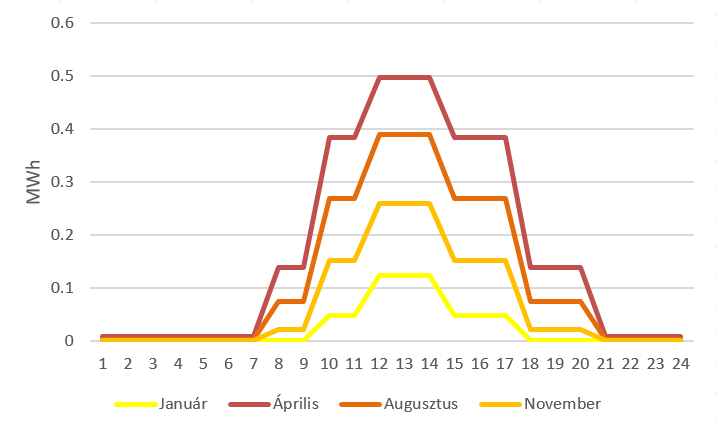
\includegraphics[scale=1.1]{PV_term_profil_abra}
    \caption{Feltételezett termelési profilok az év különböző időszakaiban, forrás: \idxsc{eemm} adatok}
    \label{fig:profilok}
\end{figure}

A számításhoz természetesen elvégezhető lenne a profil becslése általam is,
a legújabb rendelkezésre álló adatok alapján.
Ebben az esetben azonban más termelési értékek kerülnének
az egyes órák esetén az \idxsc{lcoe} számításba,
mint az árampiaci modellbe, ami a módosított \idxsc{lcoe} számításhoz
az áradatokat szolgáltatja majd (lásd lent).

Ennek oka, hogy az \idxsc{eemm} modellben napon belül csak 4 óratípus
különböztethető meg (ettől válnak a profilok lépcsőssé),
így a lentieknél pontosabb görbék nem illeszthetőek be.
Ezért döntöttem úgy, hogy az \idxsc{eemm} modellben szereplő görbéket
használom a költségbecslésem esetén is,
ugyanis így az áramárakra vonatkozó becslések és
az \idxsc{lcoe} számítás konzisztens marad. 
\label{konz}

Mindezeket figyelembe véve a saját számításom szerint 
\aref{fig:sajat}.~ábrán szemléltetett értékek adódtak.

\begin{figure}
    \centering
    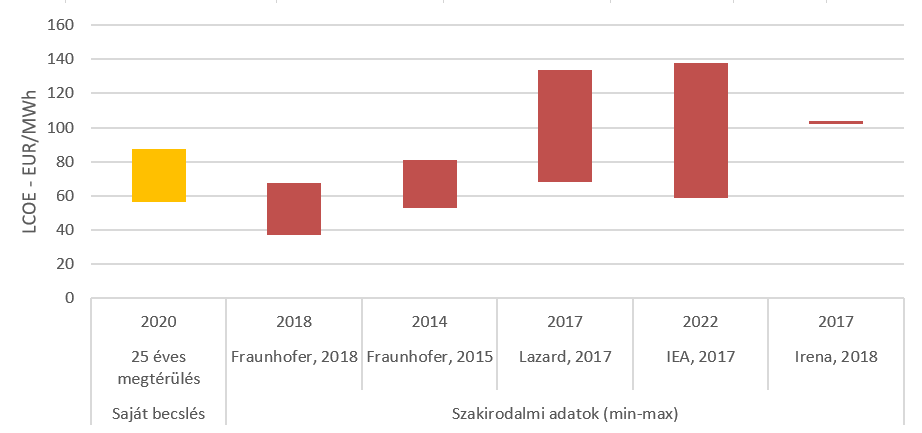
\includegraphics[scale=.85]{LCOE_sima}
    \caption{Saját \idxsc{lcoe} becslés a szakirodalom tükrében, forrás: Fraunhofer, 2018; Fraunhofer, 2015; Lazard, 2017; IEA, 2017; Irena, 2018; \idxsc{eemm} adatok}
    \label{fig:sajat}
\end{figure}

Látható, hogy a különböző források is igen nagy eltéréseket mutatnak,
illetve sok esetben igen széles sávban szóródnak a becsült értékek.
Az általam a felső táblázatban bemutatott inputokkal kalkulált érték
70 €/MWh-nak adódott, ceteris paribus magasabb
\idxsc{wacc} (7\%) esetén ez a szám 88 €/MWh,
alacsonyabb beruházási költség mellett (600 000 €/MW) pedig 56 €/MWh. 

25 év helyett 20 éves megtérülési időt feltételezve (szintén ceteris paribus)
78 €/MWh-os \idxsc{lcoe} értéket kaptam.
A számok a szakirodalom által becsült sávokba esnek,
a nemzetközi fókuszú tanulmányok alsóbb, míg a német Fraunhofer által
készített becslések felsőbb értékeihez állnak közel.


\section{Módosított \idxsc{lcoe} számítás}

Az általam vizsgált aukciós modellben a fenti logika szerint számolt
\idxsc{lcoe} érték nem értelmezhető egy az egyben úgy,
mint a szereplők költsége (vagy maradva az eredeti terminológiánál: értékelése).
Ennek oka egyrészt, hogy a támogatás itt nem egy minden egyes
megtermelt egység áram után járó fix összeg,
csak az értékesített áram piaci árát kiegészítő prémium.
Másrészt a támogatási időszak és a projekt élettartama sem egyezik meg. 

\chapter{Az aukcióelméleti modell}

\scwords Az aukcióelmélet rendkívül divatosnak mondható tudományterület,
az utóbbi évek során több, szorosan kapcsolódó részterületen tevékenykedő
közgazdász részesült Nobel-díjban. Míg a játékelmélet, illetve az aszimmetrikus
információ melletti döntések vizsgálata már korábban is középpontba került
(Selten, Nash és Harsányi 1994-es, és Mirrlees és Vickrey 1996-os díjával,
majd Aumann és Schelling 2005-ös jutalmazásával), a mechanizmustervezés
valamivel később (Hurwicz, Maskin, Myerson, 2007), a szerződéselmélet
pedig pár éve került fel a díjjal jutalmazott tudományterületek térképére
(Hart, Holmström, 2016). 2020-ban pedig Milgrom és Wilson 
,,Az árverések elméleteiért'' vehette át a díjat, munkájuk során
az aukciók gyakorlati életben történő alkalmazásáért tettek rengeteget
(pl. amerikai frekvencia kiosztási aukciók a telefontársaságok között).

Az aukcióelmélet alapjainak lefektetése Vickrey nevéhez kötődik,
és 1961-es cikke (Vickrey, 1961) óta rendkívül sokat fejlődött.
Az 1980-as évektől kezdődően rengeteg tétel egyre általánosabb
keretek közötti bizonyítása történt meg. A tudományterület
relatív fiatal, az alapvető elméleti keretrendszer azonban az
évek során kikristályosodott, és a szokásos feltevések köre –
bár egyre bővült és általánosabbá vált – jól behatárolható.
Az általános elméleti keretrendszerhez kapcsolódóan alapvető
munka (Krishna, 2010) Auction theory című könyve,
mely legtöbb fejezetében a független értékelésű aukciókkal foglalkozik.
A témával foglalkozó cikkek nagy részében az ott bemutatott
modellek tekinthetőek kiindulópontnak, én is ez alapján indulok
el a modellem felépítésekor.

A könnyebb érthetőség kedvéért a releváns szakirodalom
részletesebb ismertetése előtt néhány alapfogalmat definiálok
(a definíciókat itt is, és később is Krishna (2010) munkáját alapul véve ismertetem):

\begin{itemize}
    \item
    Kikiáltó: Az aukció kiírója, az eredeti aukcióelméleti keretrendszerben
az aukcióra bocsátott termékek eladója, az általam vizsgált esetben
azonban ő lesz a vásárló, és az aukció résztvevői kínálnak számára termékeket.
    \item
    Értékelés: az eredeti keretrendszerben az a hasznosság, amit a szereplők számára
jelent az aukcióra bocsátott tárgy megszerzése. Az általam vizsgált rendszerben éppen fordítva,
az a költség, amit a szereplők számára jelent a kínált termék biztosítása.
Vagyis legalább akkora összeget szeretnének kapni a kikiáltótól a kínált termékért cserébe,
amekkorával már kompenzálható a fellépő költség miatti hasznosságcsökkenésük.
    \item
    Ajánlati függvény (vagy Licitfüggvény): a függvény minden egyes értékelés esetén
megadja, hogy az adott szereplő milyen ajánlatot fog adni az aukción az adott értékelés esetén.
A szereplőkre vonatkozóan jellemzően nem egy értékelést, hanem egy értékeléseloszlást feltételezünk,
ezért van értelme a különböző értékelésekre egy függvényt definiálni, hiszen az adott eloszlásból
származó különböző értékelésrealizációkhoz különböző ajánlatok tartozhatnak.
Az ajánlati függvény jeleníti meg a szereplők stratégiáját.   
\end{itemize}

\chapter{Az egyensúly megkeresése}
\label{Nash}

\scwords Az egyensúly-keresési mechanizmust,
melyet a dolgozatomban alkalmazok
röviden már ismertettem a korábbi fejezetekben. Ebben a részben
részletesen is bemutatom a módszert, és ismertetem a pontos számításokat,
valamint az iteráció egyes lépései során kapott eredményeket.
Az egyenáras és az ajánlati áras aukció szignifikánsan eltér egymástól,
hiszen ahogy látni fogjuk egészen más ajánlatadási stratégia jellemzi a két aukciótípust.
Ezért a két szabályrendszert külön vizsgálom.

\section{Egyenáras aukció}\label{uniform}

Ahogy korábban kitértem rá, az egyenáras aukció esetén nincs szükség
bonyolult optimalizációs algoritmus alkalmazására. 
Egy egyszerű logika mentén levezethető a szereplők
optimális stratégiája -- függetlenül a többiek ajánlataitól.
Ez a gondolatsor a következő.

\chapter{Eredmények}\label{results}

\scwords Az egyenáras és az ajánlati áras
aukciók lejátszására, és az
eredmények kiértékelésére ebben a fejezetben
kerül sor. Az egyensúlyi stratégiákat
feltételezve szimulálom le az aukciók lejátszását,
1000--1000 alkalommal. A jobb összevethetőség kedvéért
ugyanazt a 1000*100 értékelést használom
mindkét lejátszás esetén. 

A kisorsolt értékelések mellett a megfelelő ajánlati
függvényt feltételezve -- ez az egyenáras esetben
az identitás függvény, az ajánlati áras esetben
pedig az iterációból adódó értékelés-ajánlat
párokra illesztett függvény --
minden szereplő beadja az ajánlatát,
ezekből kiválasztom a nyerteseket (mindkét aukción
a 40 legkisebb ajánlatot adó játékos nyer), meghatározom
az egyes szereplők által elnyert támogatási szintet,
és a teljes kifizetést is -- ami jelen esetben a szakirodalomban
kikiáltó bevételeként emlegetett összeg, de ez most egy
,,negatív bevétel'', hiszen beszerzési aukcióról van szó,
vagyis a kikiáltó összeköltségéről beszélhetünk.

A kapott eredményeket (legkisebb és legnagyobb nyertes ajánlat,
összes kifizetés) összevetem a korábbi német aukciók
eredményeivel is, szemelőtt tartva, hogy jelen modellezési
keretben nem tudtam minden valós körülményt figyelembe venni.
Mivel a költségbecslésem alapjául szolgáló szakirodalom
és adatok nagy része nem 2019-re vonatkozott, így 
fontosnak tartom a korábbi évek aukcióin kialakuló 
árakkal való összevetést is, hiszen az iparágban
rendkívül gyors ütemű költségcsökkenés figyelhető meg.

\section{Egyenáras aukció}

Ahogy fent bemutattuk, az egyenáras aukció esetén a stratégia megtalálása
a korábbi irodalmi eredményekre alapozva nem jelent kihívást.
Minden szereplő az értékelésének megfelelő ajánlatot ad, 
tehát az eredmények esetén nem érdemes külön foglalkozni
a kapott Nash-egyensúlyi licitfüggvénnyel, tudjuk, hogy
az identitásfüggvény a Nash-egyensúlyi ajánlatadási stratégia.
Ezért az eredmények bemutatása a kialakuló árakra 
és a kikiáltó várható összköltségére korlátozódik.
Ezek lesznek a viszonyítási pontok az ajánlati áras aukció vizsgálatakor.

Ahogy emíltettem, ahhoz, hogy a fentieket meghatározzam ismét szimulációt használok.
Az aukciót 1000 alkalommal ,,játszom le'', vagyis ennyiszer
szimulálok 100 szereplőnek beruházási költséget, és számítom ki ebből
mindegyikük $LCOE'$ értékét (vagyis értékelését).
Mivel ezen értékek
maguk az ajánlatok is, következő lépésként sorbarendezem őket,
és a legalacsonyabb 40 értékeléssel rendelkező játékost választom nyertesnek.
A kialakuló ár a 41. legalacsonyabb ajánlat, vagyis a legalacsonyabb 
már nem nyertes ajánlat, ezt a támogatási szintet kapja minden nyertes szereplő.
A kapott eredmények alapján a legalacsonyabb kialakuló 
támogatási szint 64,8 €/MWh, a legmagasabb 71,6 €/MWh,
átlagosan pedig ez az érték 68,4 €/MWh-nak adódott.

\chapter{Összefoglalás}

\scwords Dolgozatomban a német naperőművi aukciókat modellezem.
A szakirodalomban viszonylag friss területnek számít
a megújuló energia támogatásának kiosztására
vonatkozó aukciók elemzése, hiszen az ilyen típusú
tenderek néhány ország kivételével csak az elmúlt 5-10
év során tűntek fel. Németországban a pár évvel korábbi
pilot tenderek után az aukciókat a 2010-es évek második felében
kezdték el rendszeresen megszervezni, mára már számos
aukció zárult sikeresen. Ezért megfelelő terepet biztosít
az elemzésre, hiszen egyrészről az aukciós mechanizmus
már kiforrottnak mondható, másrészt kellő adat
áll rendelkezésre ahhoz is, hogy a modellezés során
kapott eredményeket összevethessem a valósakkal.

A disszertáció kutatási kérdései részben elméleti jellegűek,
a megújuló aukciók általános modellezési keretrendszeréhez
kapcsolódnak (Hogyan található meg a Nash-egyensúly,
vagy egy ahhoz közeli ajánlatadási stratégia?),
de ezeket is konkrétan a német naperőművi
aukciók esetén vizsgálom. A kérdések egy másik része
konkrét számításokkal alátámasztott, gyakorlati eredmény
(például a módosított \idxsc{lcoe'} számítás, és az ebből
kapott eloszlás).
 
Gyakorlati relevanciájuk
azért jelentős, mert a jövőben számos Európai Uniós
tagállom fog ilyen típusú aukciókat rendezni
(köztük hazánk is: 2019 szeptemberében került
sor az első, pilot aukció kiírására itthon, azóta a 2020-as
év folyamán már a második aukciót is lebonyolították), ezért
az aukciós viselkedés minél pontosabb modellezése
lehetővé teszi a döntéshozók számára, hogy megfelelő
becslést adjanak a költségvetésre vonatkozóan, 
illetve a számukra legkedvezőbb aukciós szabályrendszert állítsák fel.

\begin{thebibliography}{99}
\interlinepenalty=10000

\bibitem{Armantier-1998}
Armantier, O., Florens, J. P., \& Richard, J. F. (1998): Empirical game theoretic models: constrained equilibrium and simulation. Institut d'économie industrielle. Műhelytanulmány, frissítve 2003-ban, SUNY at Stony Brook, University of Toulouse and IDEI, University of Pittsburgh. letöltve 2021.01.14
\url{https://www.researchgate.net/profile/Jean\_Francois\_Richard2/publication/237745938\_EMPIRICAL\_GAME\_THEORETIC\_MODELS\_CONSTRAINED\_EQUILIBRIUM\_SIMULATIONS/links/54c654c60cf219bbe4f829bf.pdf}

\bibitem{Anatolitis-2016}
Anatolitis, V. (2016): Simulation of Onshore Wind Power Auctions in Germany Considering Different Auction Designs – an Agent Based Model, Master Thesis, Karlsruhe Institute of Technology and  Technical University of Vienna

\bibitem{Anatolitis-2017}
Anatolitis, V., \& Welisch, M. (2017): Putting renewable energy auctions into action–An agent-based model of onshore wind power auctions in Germany. Energy Policy, 110, 394-402.

\bibitem{Angelus-2001}
Angelus, A. (2001): Electricity price forecasting in deregulated markets. The Electricity Journal, 14(3), 32-41.

\bibitem{Atalay-2017}
Atalay, Y.,, Kalfagianni, A., \& Pattberg, P. (2017): ,,Renewable energy support mechanisms in the Gulf Cooperation Council states: Analyzing the feasibility of feed-in tariffs and auction mechanisms.'' Renewable and Sustainable Energy Reviews 72 (2017): 723-733.

\bibitem{Bartek-2019}
Bartek-Lesi, M., Mezősi, A., Pató, Z., Szabó, L., \& Szajkó, G. (2019). Megújulóenergia-felhasználás Magyarországon–a későn jövők előnye?= Renewable energy use in Hungary–The benefit of latecomers?. Vezetéstudomány-Budapest Management Review, 50(ksz.), 46-60.

\bibitem{Bartek_2019b}
Bartek-Lesi, M., Mezősi, A., Szabó, L. (2019) Sikeres aukció, de van még hova fejlődni? - Az első magyar megújulóenergia tender előzetes eredményei*, blogbejegyzés, letöltve: 2021.02.10
\url{https://metazsul.blog.hu/2019/12/11/sikeres\_aukcio\_de\_van\_meg\_hova\_fejlodni\_az\_elso\_magyar\_megujuloenergia\_aukcio\_elozetes\_eredmenyeirol}

\bibitem{Blucher-2018}
Blücher, F. von, Gephart, M., Wigand, F., Anatolitis, V., Winkler, J., Held, A., Sekamane, J. K. \& Kitzing, L. (2018): AURES II report D6.1: Design options for cross-border auctions, letöltve: 2019.10.02., 
\url{http://aures2project.eu/wp-content/uploads/2019/06/AURES_II_D6_1_final.pdf}

\bibitem{Blucher-2019}
Blücher, F. von (2019): Cross border auctions - An emerging option to cost effectively deploy renewables; AURES II Regional Workshop, Budapest, 2019. június 25., letöltve: 2019.10.02., 
\url{https://rekk.hu/downloads/events/Felix\%20von\%20Blücher\_Navigant\_Cross-boarder\%20auctions.pdf}

\bibitem{Bosshard-2017}
Bosshard, V., Bünz, B., Lubin, B., \& Seuken, S. (2017): Computing Bayes-Nash Equilibria in Combinatorial Auctions with Continuous Value and Action Spaces. In IJCAI (pp. 119-127).
letöltve: 2021.01.14
\url{https://www.ifi.uzh.ch/ce/publications/BNE\_Bosshard\_et\_al\_IJCAI\_2017-long.pdf}

\bibitem{Bouallegue-2013}
Bouallègue, F. B., Crouzet, J. F., \& Mariano-Goulart, D. (2013): A heuristic statistical stopping rule for iterative reconstruction in emission tomography. Annals of nuclear medicine, 27(1), 84-95.
letöltve: 2021.01.14
\url{https://link.springer.com/article/10.1007/s12149-012-0657-5}

\bibitem{Bundes-2019}
Bundesministerium der Justiz und für Verbraucherschutz (2019): Gesetz für den Ausbau erneuerbarer Energien (Erneuerbare-Energien-Gesetz - EEG 2017), 2019. május 13-án módosított változat, 2019. októberében is hatályos verzió, letöltve: 2019.10.02, 
\url{https://www.gesetze-im-internet.de/eeg\_2014/BJNR106610014.html}

\bibitem{Bundes-219a}
Bundesnetzagentur (2019): Ausschreibungen 2019, Napelemaukciókról szóló statisztikák, letöltve: 2019.10.03., 
\url{https://www.bundesnetzagentur.de/DE/Sachgebiete/ElektrizitaetundGas/Unternehmen\_Institutionen/Ausschreibungen/Solaranlagen/BeendeteAusschreibungen/BeendeteAusschreibungen\_node.html}

\bibitem{Chen-2005}
Chen, Y., \& Hobbs, B. F. (2005). An oligopolistic power market model with tradable NO/sub x/permits. iEEE Transactions on Power systems, 20(1), 119-129.

\bibitem{Conejo-2005}
Conejo, A. J., Plazas, M. A., Espinola, R., \& Molina, A. B. (2005): Day-ahead electricity price forecasting using the wavelet transform and ARIMA models. IEEE transactions on power systems, 20(2), 1035-1042.

\bibitem{Cretu-2019}
Cretu, Gabriela (2019): RES Auctions in the Energy Community, előadva: 2nd AURES II Regional Workshop Renewable Energy Auctions in Austria - Best Practices and Impact Mitigation, 2019. november 22, Bécs

\bibitem{Hlouskova-2004}
CELEX:32009L0028uaresma, J. C., Hlouskova, J., Kossmeier, S., \& Obersteiner, M. (2004): Forecasting electricity spot-prices using linear univariate time-series models. Applied Energy, 77(1), 87-106.
de Keijzer, B., Markakis, E., Schäfer, G., \& Telelis, O. (2013): Inefficiency of standard multi-unit auctions. In European Symposium on Algorithms (pp. 385-396). Springer, Berlin, Heidelberg.

\bibitem{delRio-2014}
del Río, P., \& Linares, P. (2014): Back to the future? Rethinking auctions for renewable electricity support. Renewable and Sustainable Energy Reviews, 35, 42-56.

\bibitem{delRio-2017a}
del Río, P. (2017a): AURES Report D4.4-ZM,  Auctions for Renewable  Support in Zambia: Instruments and lessons learnt, letöltve: 2019.05.25,
\url{http://auresproject.eu/sites/aures.eu/files/media/documents/zambia\_final.pdf}

\bibitem{delRio-2017b}
del Río, P. (2017b): AURES Report D4.4-PE, Auctions for Renewable Support in Peru: Instruments and lessons learnt, letöltve: 2019.05.25
\url{http://auresproject.eu/sites/aures.eu/files/media/documents/peru\_final.pdf}

\bibitem{Diallo-2019}
Diallo, A., Dézsi, B., Denková, A., Jakóbik, W., Jordanova, A., Kácsor, E., Madleňák, T., Misik, M., Moskwik, K.,
Oravcova, V., Roszkowski, M., Szabó, L., Takácsné Tóth, B., Törőcsik, Á. (2018): ‘Beyond gas’ – energy security issues in the V4 after 2020, Final Synthesis Report,
Letöltve: 2019.11.03,
\url{http://www.amo.cz/wp-content/uploads/2018/12/V4-Beyond-Gas-Beyond-2020-Final-Synthesis-Report.pdf}

\bibitem{entso}
ENTSO-E: Transparency Platform,
\url{https://transparency.entsoe.eu/}

\bibitem{entso-2015}
ENTSO-E (2015): Europe’s  future  secure and  sustainable  electricity  infrastructure, e-Highway2050 project results, 
\url{https://docs.entsoe.eu/baltic-conf/bites/www.e-highway2050.eu/e-highway2050/}

\bibitem{entso-2018}
ENTSO-E (2018): Ten Year Network Development Plan, 
\url{https://tyndp.entsoe.eu/}

\bibitem{eb-2019}
Európai Bizottság (2009): Az Európai Parlament és a Tanács 2009/28/ek irányelve (2009. április 23.) a megújuló energiaforrásból előállított energia támogatásáról, valamint a 2001/77/EK és a 2003/30/EK irányelv módosításáról és azt követő hatályon kívül helyezéséről, letöltve: 2019.05.25., 
\url{https://eur-lex.europa.eu/legal-content/HU/TXT/PDF/?uri=CELEX:32009L0028\&from=EN}

\bibitem{eb-2014}
Európai Bizottság (2014): Iránymutatás a 2014–2020 közötti időszakban nyújtott környezetvédelmi és energetikai állami támogatásokról (2014/C 200/01), 
\url{https://eur-lex.europa.eu/legal-content/HU/TXT/PDF/?uri=CELEX:52014XC0628(01)\&from=EN}

\bibitem{eb-2016}
    Európai Bizottság (2016): EU Reference Scenario 2016 Energy, transport and GHG emissions Trends to 2050, letöltve: 2019.05.26.,
    \url{https://ec.europa.eu/energy/sites/ener/files/documents/20160713\%20draft\_publication\_REF2016\_v13.pdf}

\bibitem{ep-2018}
Európai Parlament és a Tanács (2018): Az Európai Parlament és a Tanács (EU) 2018/1999 rendelete, az energiaunió és az éghajlat-politika irányításáról, valamint a 663/2009/EK és a 715/2009/EK európai parlamenti és tanácsi rendelet, a 94/22/EK, a 98/70/EK, a 2009/31/EK a 2009/73/EK, a 2010/31/EU, a 2012/27/EU és a 2013/30/EU európai parlamenti és tanácsi irányelv, a 2009/119/EK és az (EU) 2015/652 tanácsi irányelv módosításáról, továbbá az 525/2013/EU európai parlamenti és tanácsi rendelet hatályon kívül helyezéséről,
letöltve: 2020.02.01, 
\url{https://eur-lex.europa.eu/legal-content/HU/TXT/PDF/?uri=CELEX:32018R1999&from=EN} 

\bibitem{et-2014}
Európai Tanács (2014): Conclusions - 23/24 October 2014, letöltve: 2019.05.25.
\url{https://www.consilium.europa.eu/uedocs/cms\_data/docs/pressdata/en/ec/145397.pdf}

\bibitem{eurostat-2021}
Eurostat (2021): SHARES database, datatable: Share of energy from renewable sources, letöltve: 2021.01.15,
\url{https://ec.europa.eu/eurostat/web/energy/data/shares}

\bibitem{Fabra-2019}
Fabra, N., von der Fehr, N.-H., \& Harbord, D. (2002): Designing Electricity Auctions: Uniform, Discriminatory and Vickrey. Letöltve: 2019.05.17,
\url{http://citeseerx.ist.psu.edu/viewdoc/download?doi=10.1.1.297.1810\&rep=rep1\&type=pdf}

\bibitem{Frederico-2003}
Federico, G., \& Rahman, D. (2003): Bidding in an electricity pay-as-bid auction. Journal of Regulatory Economics, 24(2), 175-211.

\bibitem{Foxon-2005}
Foxon, T. J., Gross, R., Chase, A., Howes, J., Arnall, A., \& Anderson, D. (2005). UK innovation systems for new and renewable energy technologies: drivers, barriers and systems failures. Energy policy, 33(16), 2123-2137.

\bibitem{Fraunhofer-2015}
Fraunhofer ISE (2015): Current and Future Cost of Photovoltaics. Long-term Scenarios for Market Development, System Prices and LCOE of Utility-Scale PV Systems. Study on behalf of Agora Energiewende, letöltve: 2019.05.25.
\url{https://www.ise.fraunhofer.de/content/dam/ise/de/documents/publications/studies/AgoraEnergiewende\_Current\_and\_Future\_Cost\_of\_PV\_Feb2015\_web.pdf}

\bibitem{Fraunhofer-2018}
Fraunhofer (2018): Levelized Cost Of Electricity, Renewable Energy Technologies, March 2018, letöltve: 2019.05.25.
\url{https://www.ise.fraunhofer.de/en/publications/studies/cost-of-electricity.html}

\bibitem{Fraunhofer-2019}
Fraunhofer (2019): Energy charts database, Net installed electricity generation capacity in Germany, letöltve:
\url{2019.10.02, https://www.energy-charts.de/power\_inst.htm}

\bibitem{Garcia-2205}
Garcia, R. C., Contreras, J., Van Akkeren, M., \& Garcia, J. B. C. (2005): A GARCH forecasting model to predict day-ahead electricity prices. IEEE transactions on power systems, 20(2), 867-874.

\bibitem{Gkm-2002}
Gazdasági és Közlekedési Minisztérium (2002): 56/2002. (XII. 29.) GKM rendelet 
az átvételi kötelezettség alá eső villamos energia átvételének szabályairól és árainak megállapításáról, letöltve: 2019.09.30, 
\url{http://www.panenerg.hu/webimages/files/56\_2002\_GKM\_rendelet.pdf}

\bibitem{Guth-2005}
Güth, W., R. Ivanova-Stenzel \& E. Wolfstetter (2005): “Bidding Behavior in Asymmetric Auctions: An Experimental Study,” European Economic Review 49:1891-1913.

\bibitem{Hailu-2206}
Hailu, A., \& Thoyer, S. (2006): Multi-unit auction format design. Journal of Economic Interaction and Coordination, 1(2), 129-146.),

\bibitem{Haufe-2018}
Haufe, M. C., \& Ehrhart, K. M. (2018): Auctions for renewable energy support–Suitability, design, and first lessons learned. Energy policy, 121, 217-224.

\bibitem{Higgins_2010}
Higgins, N. A. (2010): Computational and Experimental Market Design (Doktori értekezés), University of Maryland, letöltve: 2021.01.14
\url{https://drum.lib.umd.edu/handle/1903/10260}

\bibitem{Hudson-2000}
Hudson, R. (2000): Analysis of uniform and discriminatory price auctions in restructured electricity markets. Oak Ridge National Laboratory, Oak Ridge, TN.

\bibitem{Iea-2015}
IEA (2015): Projected Costs of Generating Electricity, 2015 Edition, Paris, France (letöltve: 2017.05.26),
\url{https://www.oecd-nea.org/ndd/pubs/2015/7057-proj-costs-electricity-2015.pdf}

\bibitem{Iea-2017}
IEA (2017): Renewables 2017, Analysis and Forecasts to 2022, letöltve:
\url{2019.05.26 https://www.iea.org/renewables2017/}

\bibitem{Iea-2018}
IEA (2018): Trends 2018 in photovoltaic applications Report IEA PVPS T1-34:2018, letöltve: 2019.05.26.
\url{http://www.iea-pvps.org/fileadmin/dam/intranet/task1/IEA\_PVPS\_Trends\_2018\_in\_Photovoltaic\_Applications\_03.pdf}

\bibitem{Irena-2016}
IRENA (2016): The Power To Change: Solar And Wind Cost Reduction PotentiaL to 2025, International Renewable Energy Agency, Bonn, Germany, 2016., letöltve: 2019.05.26,
\url{https://www.irena.org/publications/2016/Jun/The-Power-to-Change-Solar-and-Wind-Cost-Reduction-Potential-to-2025}

\bibitem{Irena-2018}
IRENA (2018): Renewable Power Generation Costs in 2017, letöltve: 2019.05.26.
\url{http://www.irena.org/publications/2018/Jan/Renewable-power-generation-costs-in-2017}

\bibitem{Itaba-2018}
Itaba, S.,\& Mori, H. (2017): A Fuzzy-Preconditioned GRBFN Model for Electricity Price Forecasting. Procedia Computer Science, 114, 441-448.

\bibitem{Iychettira-2017}
Iychettira, K., Hakvoort, R., Linares, P., \& Jeu, R. (2017): Towards a comprehensive policy for electricity from renewable energy: designing for social welfare, Applied Energy, Volume 187, 1 February 2017, Pages 228–242

\bibitem{Iychettira-2017a}
Iychettiraa K., Hakvoort, R., \& Linares, P. (2017): Towards a comprehensive policy for electricity from renewable energy: An approach for policy design, Energy Policy, Volume 106, July 2017, Pages 169–182

\bibitem{Jakasa-2011}
Jakaša, T., Andročec, I., \& Sprčić, P. (2011, May): Electricity price forecasting—ARIMA model approach. In Energy Market (EEM), 2011 8th International Conference on the European (pp. 222-225). IEEE.

\bibitem{Jensen-2008}
Jensen, S. G., \& Meibom, P. (2008). Investments in liberalised power markets: Gas turbine investment opportunities in the Nordic power system. International Journal of Electrical Power \& Energy Systems, 30(2), 113-124.

\bibitem{Kacsor-2019}
Kácsor, E., Kerekes, L., \& Mezősi, A. (2019). Egy sikeres piacnyitás története? Liberalizáció a magyar villamosenergia-szektorban= Is it a history of a successful market opening? Liberalization in the Hungarian electricity sector. Vezetéstudomány-Budapest Management Review, 50(ksz.), 19-31.

\bibitem{Kacsor-2020}
Kácsor, E. (2020) Hatékony kiosztás a nagyoknál, sok érvénytelen pályázat a kicsiknél, Végleges METÁR eredmények, blogbejegyzés, letöltve: 2021.02.10
\url{https://metazsul.blog.hu/2020/04/01/hatekony\_kiosztas\_a\_nagyoknal\_sok\_ervenytelen\_palyazat\_a\_kicsiknel?token=8441d8e712dbe1b31009ea4266ec76e4}

\bibitem{Keles-2016}
Keles, D., Scelle, J., Paraschiv, F., \& Fichtner, W. (2016): Extended forecast methods for day-ahead electricity spot prices applying artificial neural networks. Applied energy, 162, 218-230.

\bibitem{Klemperer-1999}
Klemperer, P. (1999): Auction Theory: A guide to the literature (Vol. 13) (No. 3).

\bibitem{Klobasa-2018}
Klobasa, M. \& Ragwitz, M. (2018): Diskussionspapier Contract for Difference Regime (CfD) – Mo gliche Ausgestaltungen, Karlsruhe, Fraunhofer

\bibitem{Kormany-2017}
Kormány (2007): 389/2007. (XII. 23.) Korm. rendelet a megújuló energiaforrásból vagy hulladékból nyert energiával termelt villamos energia, valamint a kapcsoltan termelt villamos energia kötelező átvételéről és átvételi áráról, letöltve: 2019.09.30,
\url{http://njt.hu/cgi\_bin/njt\_doc.cgi?docid=112846.293540}

\bibitem{Kotek-2016}
Kotek, P. (2016): Honnan fúj? A szélerőműveket érintő szabályozás változásairól. letöltve: 2019.09.30,
\url{https://rekk.hu/downloads/academic\_publications/rekk\_policybrief\_2016\_05.pdf}

\bibitem{Keh-2019}
Köztársasági Elnöki Hivatal (2019): Áder János köztársasági elnök beszéde az ENSZ-klímacsúcson New Yorkban, az ENSZ székházában, letöltve: 2019.10.01.,
\url{https://www.keh.hu/beszedek/2681-Ader\_Janos\_koztarsasagi\_elnok\_beszede\_az\_ENSZ\_klimacsucson\_New\_Yorkban\_az\_ENSZ\_szekhazaban\&pnr=1}

\bibitem{Kreiss-2017}
Kreiss, J., Ehrhart, K., \& Haufe, M. (2017): ,,Appropriate design of auctions for renewable energy support–Prequalifications and penalties.'' Energy Policy 101, 512-520.

\bibitem{Krishna-2010}
Krishna, V. (2010): Auction theory – Second edition, Elsevier, London, UK

\bibitem{Kumar-2018}
Kumar, V., Singh, N., Singh, D. K., \& Mohanty, S. R. (2018): Short-Term Electricity Price Forecasting Using Hybrid SARIMA and GJR-GARCH Model. In Networking 

\bibitem{Kylili-2015}
Kylili, A., Fokaides, P. A. (2015): Competitive auction mechanisms for the promotion renewable energy technologies: The case of the 50 MW photovoltaics projects in Cyprus, Renewable and Sustainable Energy Reviews 42 (2015) 226–233 pp

\bibitem{Lazard-2017}
Lazard (2017): Lazard’s Levelized Cost of Energy analysis – Version 11.0, letöltve: 2019.05.26.
\url{https://www.lazard.com/media/450337/lazard-levelized-cost-of-energy-version-110.pdf}

\bibitem{Luo-2015}
Luo, X., Stordal, A. S., Lorentzen, R. J., \& Naevdal, G. (2015): Iterative ensemble smoother as an approximate solution to a regularized minimum-average-cost problem: theory and applications. arXiv preprint arXiv:1505.01135. letöltve: 2021.01.14
\url{https://arxiv.org/pdf/1505.01135.pdf}

\bibitem{Marshall-1994}
Marshall, R. C., Meurer, M. J., Richard, J. F., \& Stromquist, W. (1994): Numerical analysis of asymmetric first price auctions. Games and Economic behavior, 7(2), 193-220.
letöltve: 2021.01.14
\url{https://www.sciencedirect.com/science/article/abs/pii/S0899825684710451}

\bibitem{McAfee-1987}
McAfee, R. P., \& McMillan, J. (1987): Auctions and bidding. Journal of economic literature, 25(2), 699-738.)

\bibitem{Mekh-2016}
MEKH (2016): 17/2016 MEKH rendelet a megújuló energiaforrásokból termelt villamos energia működési támogatásának mértékéről, letöltve: 2017.05.26,
\url{https://net.jogtar.hu/jr/gen/hjegy\_doc.cgi?docid=A1600017.MEK\&timeshift=fffffff4\&txtreferer=00000001.TXT}

\bibitem{Mekh-2019}
MEKH (2019): Pályázati kiírási dokumentáció, Megújuló energiaforrásból termelt villamos energia támogatása pályázati zöld prémium rendszer keretében, letöltve: 2019.10.01,
\url{http://www.mekh.hu/download/fix/metar\_kiirasi\_dokumentacio\_20190902}

\bibitem{Mekh-2020}
MEKH(2020): A 2020-as METÁR-pályázat bontási adatai, letöltve: 2021.02.10
\url{http://www.mekh.hu/a-2020-as-metar-palyazat-bontasi-adatai}

\bibitem{Mezosi-2016}
Mezősi, A., \& Szabó, L. (2016). Model based evaluation of electricity network investments in Central Eastern Europe. Energy Strategy Reviews, 13, 53-66.

\bibitem{Mezosi-2017a}
Mezősi, A., Pató, Zs. \& Szabó, L. (2017a): Meg-megújuló statisztikák, REKK Policy brief, 2017/1, letöltve: 2019.10.01,
\url{https://rekk.hu/downloads/academic\_publications/rekk\_policybrief\_hu\_2017\_01.pdf}

\bibitem{Mezosi-2017b}
Mezősi, A., Kácsor, E., Beöthy, Á., Törőcsik, Á., \& Szabó, L. (2017b). Modelling support policies and renewable energy sources deployment in the Hungarian district heating sector. Energy \& Environment, 28(1-2), 70-87.

\bibitem{Mezosi-2018}
Mezősi, A., Szabó, L., \& Szabó, S. (2018). Cost-efficiency benchmarking of European renewable electricity support schemes. Renewable and Sustainable Energy Reviews, 98, 217-226.

\bibitem{Mezosi-2019}
Mezősi, A., Bartek-Lesi, M., Dézsi, B., Diallo, A., Kácsor, E., Kerekes, L., Kotek, P., Mészégetőné Keszthelyi, A., Rácz, V., Selei, A., Szajkó, G., Szabó, L., \& Vékony, A. 2019): A hazai nagykereskedelmi villamosenergia-piac modellezése és ellátásbiztonsági elemzése 2030-ig különböző erőművi forgatókönyvek mellett, REKK, 
\url{https://rekk.hu/downloads/projects/2019\_Arampiac\_REKK.pdf}

\bibitem{Milgrom-1982}
Milgrom, P. R., \& Weber, R. J. (1982): A Theory of Auctions and Competitive Bidding (Vol. 50) (No.5). Letöltve: 2019.05.17, 
\url{http://www.jstor.org/stable/1911865?origin=crossref}, doi: 10.2307/1911865

\bibitem{Morgan-2001}
Morgan, J. (2001): Efficiency in auctions: theory and practice.
Updated copies of this paper can be found at
\url{www. wws. princeton. edu/~rjmorgan}. Journal of International Money and Finance, 20(6), 809-838.

\bibitem{Mori-2016}
Mori, H., \& Nakano, K. (2016): An Efficient Hybrid Intelligent Method for Electricity Price Forecasting. Procedia Computer Science, 95, 287-296.

\bibitem{Naroditskiy-2007}
Naroditskiy, V., \& Greenwald, A. (2007): Using iterated best-response to find Bayes-Nash equilibria in auctions. In PROCEEDINGS OF THE NATIONAL CONFERENCE ON ARTIFICIAL INTELLIGENCE (Vol. 22, No. 2, p. 1894). Menlo Park, CA; Cambridge, MA; London; AAAI Press; MIT Press, letöltve: 2021.01.14
\url{https://www.aaai.org/Papers/AAAI/2007/AAAI07-322.pdf}

\bibitem{nm-2016}
Nemzetgazdasági Miniszter (2016): A nemzetgazdasági miniszter 34/2016. (IX. 14.) NGM rendelete a Villamosmű Műszaki-Biztonsági Követelményei Szabályzat hatályba léptetéséről szóló 8/2001. (III. 30.) GM rendelet, és a villamosművek, valamint a termelői, magánés közvetlen vezetékek biztonsági övezetéről szóló 2/2013. (I. 22.) NGM rendelet módosításáról, 

\bibitem{nfm-2011}
Nemzeti Fejlesztési Minisztérium (2011): Szabályozási koncepció a megújuló- és alternatív energiaforrásokból előállított hő- és villamos energia kötelező átvételi rendszerről, letöltve: 2019.09.30,
\url{http://metar.hu/metar\_szabalyozas\_torveny.html}

\bibitem{nfm-2016a}
Nemzeti Fejlesztési Minisztérium (2016a): 62/2016 NFM rendelet a megújuló energiaforrásból származó villamos energia termelési támogatás korlátairól és a prémium típusú támogatásra irányuló pályázati eljárásról, letöltve: 2017.05.26,
\url{https://net.jogtar.hu/jr/gen/hjegy\_doc.cgi?docid=a1600062.nfm}

\bibitem{nfm-2016b}
Nemzeti Fejlesztési Minisztérium (2016b): 63/2016 NFM rendelet a megújuló energiaforrásokból nyert energiával termelt villamos energia működési támogatásának finanszírozásához szükséges pénzeszköz mértékének megállapítási módjára és a megfizetésre vonatkozó részletes szabályokról, letöltve: 2017.05.26,
\url{https://net.jogtar.hu/jr/gen/hjegy\_doc.cgi?docid=a1600063.nfm}

\bibitem{nfm-2016c}
Nemzeti Fejlesztési Minisztérium (2016c): 55/2016 NFM rendelet a megújuló energiát termelő berendezések és rendszerek beszerzéséhez és működtetéséhez nyújtott támogatások igénybevételének műszaki követelményeiről, letöltve: 2017.05.26,
\url{https://net.jogtar.hu/jr/gen/hjegy\_doc.cgi?docid=A1600055.NFM\&timeshift=fffffff4\&txtreferer=00000001.TXT}

\bibitem{Novshek-1982}
Novshek, W., \& Sonnenschein, H. (1982): Fulfilled expectations Cournot duopoly with information acquisition and release. The Bell Journal of Economics, 214-218. letöltve: 2021.01.14
\url{https://www.jstor.org/stable/3003442?seq=1\#metadata\_info\_tab\_contents}

\bibitem{Osepayshvili-2005}
Osepayshvili, A., Wellman, M. P., Reeves, D. M. \&  MacKieMason J. K. (2005):  Self-Confirming Price Prediction for Bidding in Simultaneous Ascending Auctions. Műhelytanulmány, University of Michigan Ann Arbor, MI 48109 USA. letöltve: 2021.01.14
\url{https://drops.dagstuhl.de/opus/volltexte/2005/202/pdf/05011.MacKieMasonJeffrey.Paper.202.pdf}

\bibitem{Ostrovsky-2011}
Ostrovsky, M., \& Schwarz, M. (2011): Reserve prices in internet advertising auctions: a field experiment. EC, 11, 59-60. Letöltve: 2019.05.17.
\url{https://web.stanford.edu/~ost/papers/rp.pdf}

\bibitem{Pato-2016}
Pató, Zs. (2016): A hurok szorításában, REKK Jelentés az Energiapiacokról 2016/1, letöltve: 2019.10.02,
\url{https://rekk.hu/downloads/publications/Rekk\_jelentes\_2016\_1.pdf\#page=11}

\bibitem{Pineau-2007}
Pineau, P. O., \& Zaccour, G. (2007). An oligopolistic electricity market model with interdependent segments. The Energy Journal, 28(3), 165.

\bibitem{Rabinovich-2013}
Rabinovich, Z., Naroditskiy, V., Gerding, E.H., \& Jennings N.R. (2013): Computing pure bayesian-nash equilibria in games with finite actions and continuous types. Artificial Intelligence, 195:106–139, 2013.

\bibitem{Reeves-2004}
Reeves, D. \& Wellman, M. (2004): Computing best-response strategies in infinite games of incomplete information. In Proceedings of the 20th Conference on Uncertainty in Artificial Intelligence
(UAI), pages 470–478, 2004.

\bibitem{Reiley-2006}
    Reiley, D. H. (2006): Field experiments on the effects of reserve prices in auctions: More magic on the internet. The RAND Journal of Economics, 37(1), 195-211. Letöltve: 2019.05.17
    \url{ https://onlinelibrary.wiley.com/doi/epdf/10.1111/j.1756-2171.2006.tb00012.x}

\bibitem{res-2019}
res-legal (2019): RES Legal, Legal sources on renewable energy, Letöltve: 2019.11.03,
\url{http://www.res-legal.eu/en/home/}

\bibitem{Selei-2017}
Selei, A. (2017). Az európai fogyasztók jólétének az elemzése: Vizsgálatok gázpiaci modellezés segítségével (Doctoral dissertation, Budapesti Corvinus Egyetem).

\bibitem{Shrimali-2016}
Shrimali, G., Konda, C., \& Farooquee, A. A. (2016): ,,Designing renewable energy auctions for India: Managing risks to maximize deployment and cost-effectiveness.'' Renewable Energy 97 (2016): 656-670.

\bibitem{Singh-2017}
Singh, N., Mohanty, S. R., \& Shukla, R. D. (2017): Short term electricity price forecast based on environmentally adapted generalized neuron. Energy, 125, 127-139.

\bibitem{Sternkopf-2019}
Sternkopf, T. (2019): res-legal.eu, Tenders (Sliding feed-in premium) in Germany, letöltve: 2019.10.02,
\url{http://www.res-legal.eu/search-by-country/germany/single/s/res-e/t/promotion/aid/tenders-auctioning-the-feed-in-support-for-ground-mounted-installations/lastp/135/}

\bibitem{Sugianto-2014}
Sugianto, L. F.,\& Liao, K. Z. (2014): Comparison of different auction pricing rules in the electricity market. Modern Applied Science, 8(1), 147.

\bibitem{Szabo-2017a}
Szabó, L., Mezősi, A., Pató, Zs., Kelemen, Á., Beöthy, Á., Kácsor, E., Kaderják, P., Resch, G:, Liebmann, L., Hiesl, A., et al. (2017): South East Europe Electricity Roadmap: Country report: Albania, Budapest, Magyarország : REKK Regionális Energia- és Infrastruktúra-politikai Együttműködésért Alapítvány, 52 p., letöltve: 2020.02.01,
\url{https://rekk.hu/downloads/projects/SEERMAP_CR_ALBANIA_A4_ONLINE.pdf}

\bibitem{Szabo-2017b}
Szabó, L., Mezősi, A., Pató, Zs., Kelemen, Á., Beöthy, Á., Kácsor, E., Kaderják, P., Resch, G:, Liebmann, L., Hiesl, A., et al. (2017): South East Europe Electricity Roadmap: Regional report: South East Europe, Budapest, Magyarország : REKK Regionális Energia- és Infrastruktúra-politikai Együttműködésért Alapítvány, 64 p., letöltve: 2020.02.02,
\url{https://rekk.hu/downloads/projects/SEERMAP_RR_SEE_A4_ONLINE.pdf}

\bibitem{Szabo-2019a}
Szabó, L., Bartek-Lesi, M., Diallo, A., \& Dézsi, B. (2019): AURES – II: Cross-border  auctions – considerations for Hungary, előadva: Project Meeting 2019. november 20-21, Bécs

\bibitem{Szabo-2019b}
Szabó, L., Kelemen, Á., Mezősi, A., Pató, Z., Kácsor, E., Resch, G., \& Liebmann, L. (2019). South East Europe electricity roadmap–modelling energy transition in the electricity sectors. Climate policy, 19(4), 495-510.
\url{https://doi.org/10.1080/14693062.2018.1532390}

\bibitem{Tierney-2008}
Tierney, S. F., Schatzki, T., \& Mukerji, R. (2008): Uniform-pricing versus pay-as-bid in wholesale electricity markets: does it make a difference?. New York ISO.

\bibitem{Varga-2020a}
Varga, K. (2020b) Jönnek a hatalmas naperőműparkok? A MEKH kiírta a második METÁR-pályázatot, blogbejegyzés, letöltve: 2021.02.10
\url{https://metazsul.blog.hu/2020/08/11/jonnek\_a\_hatalmas\_naperomuparkok}

\bibitem{Varga-2020b}
Varga, K. (2020b) Egy ábrán az eddigi METÁR-aukciók, blogbejegyzés, letöltve: 2021.02.10
\url{https://metazsul.blog.hu/2020/10/27/egy\_abran\_az\_eddigi\_metar-aukciok?token=cee4e0c84a1d6c635392d03f56752174}

\bibitem{Viana-2018}
Viana, A. G., \& Ramos, D. S. (2018). Outcomes from the first large-scale solar PV auction in Brazil. Renewable and Sustainable Energy Reviews, 91, 219-228.

\bibitem{Vickrey-1961}
Vickrey, W. (1961): “Counterspeculation, Auctions, and Competitive Sealed Tenders,” Journal of Finance, 16(1), 8–37.

\bibitem{Vorobeychik-2008}
Vorobeychik, Y., Wellman, M. (2008): Stochastic search methods for nash equilibrium approximation in simulation-based games. In Proceedings of the 7th International Joint Conference on
Autonomous Agents and Multiagent Systems (AAMAS), pp 1055–1062, 2008.

\bibitem{Welisch-2016}
Welisch, M., Ortner, A., \& Resch, G. (2016). Assessment of RES technology market values and the merit-order effect–an econometric multi-country analysis. Energy \& Environment, 27(1), 105-121.

\bibitem{Welisch-2019}
Welisch, M. (2019): Multi-unit renewables auctions for small markets-Designing the Danish multi-technology auction scheme. Renewable energy, 131, 372-380.

\bibitem{Wigand-2016}
Wigand, F., Förster, S., Amazo, A., \& Tiedemann, S. (2016): AURES Report D4.2, Auctions for Renewable Energy Support: Lessons Learnt from International Experiences, letöltve: 2019.05.25, 
\url{http://auresproject.eu/sites/aures.eu/files/media/documents/aures\_wp4\_synthesis\_report.pdf}

\bibitem{Wirth-2019}
Wirth, H. (2019): Recent Facts about Photovoltaics in Germany, letöltve: 2019.10.02.,
\url{https://www.ise.fraunhofer.de/content/dam/ise/en/documents/publications/studies/recent-facts-about-photovoltaics-in-germany.pdf}

\bibitem{Zhao-2017}
Zhao, Z., Wang, C., Nokleby, M., \& Miller, C. J. (2017): Improving short-term electricity price forecasting using day-ahead LMP with ARIMA models. In Power \& Energy Society General Meeting, 2017 IEEE (pp. 1-5). IEEE.
\end{thebibliography}

\backmatter
\renewcommand{\appendixpagename}{Függelékek}
\renewcommand{\appendixtocname}{\appendixpagename}
\appendix
\appendixpage
\renewcommand{\chaptername}{\appendixname}
\chapter{Az \textsc{eemm} modell technikai specifikációja}\label{app:1}

\scwords A tökéletesen versenyző piac feltételezésből adódóan az egyensúlyi állapot a teljes modellezett
régió jólétének együttes maximalizálásával kapható – a termelők és a fogyasztók jólétei összegének
maximumát keressük minden modellezett óra esetén.
Ennek a jólétnek a számítása a következőképpen történik:

\[
    W=
    \sum_{i=1}^nTCS_m-TC
\]
A jólét tehát a bruttó fogyasztói többlet (vagyis a keresleti görbe alatti terület) és az áramtermeléshez
kapcsolódó változó költségek különbsége.
A két tétel kibontva a következőképpen írható fel:
\[
    TCS_m=
    \int_0^{Q_m}D_m^{-1}(Q)\,dQ=A_mQ_m-\frac{B_m}{2}Q_m^22\mbox{ és }
    TC=\sum_{p=1}^Pc_pq_p
\]

A fenti értékek különbségének maximumát három feltétel mellett keressük.
Minden termelőegységhez
tartozik egy kapacitáskorlát: a blokk termelése nem lehet nagyobb,
mint a kapacitása,
de nagyobb
vagy egyenlő kell, hogy legyen, mint nulla.
A második feltétel a határkeresztező kereskedelemre vonatkozik,
a szállítás nem lépheti át az adott metszék (adott irányú) kapacitását.
A harmadik feltétel pedig
a kereslet és kínálat egyensúlyára vonatkozik: a teljes fogyasztás minden piac esetén meg kell,
hogy egyezzen a hazai erőművi termelés és a nettó import (ami negatív is lehet!) összegével
minden egyes modellezett óra esetén.
(Az utolsó feltétel esetén $\delta$ értéke $1$, ha a kereskedelem $A$-ból $B$ irányába történik,
és $-1$ ellenkező esetben).

\begin{enumerate}
    \item $0\leq q_p\leq C_p$,
    \item $N_i\leq t_i\leq N_i$,
    \item $Q_m=\sum_{p}q_p+\sum_i\delta_{i,m}t_i.$
\end{enumerate}
A fentieket összefoglalva tehát a következő maximalizáció végzi a modell:
\begin{multline}
    W=\\
    \sum_{m=1}^M\left( A_m\left( \sum_pq_p+\sum_i\delta_{i,m}t_i \right)-\frac{B_m}{2}\left( \sum_pq_p+\sum_i\delta_{i,m}t_i \right)^2 \right)
    -
    \sum_{p=1}^Pc_pq_p\\
    \rightarrow \max
\end{multline}

 
Jelölések: piacok: $m=1,\ldots,M$; fogyasztás: $Q$; erőművi blokk: $p$;
erőművi termelés: $q$; változó költség: $c$; export-import áramlás: $t$;
erőművi kapacitáskorlát: $C$; kapacitáskorlát a határokon: $N$;
teljes jólét: $W$; Teljes fogyasztói többlet: $TCS$;
Villamosenergia-termelés költsége: $TC$, kereslet: $D$;
keresleti görbét meghatározó konstansok: $A$ és $B$


\chapter{Az iteráció egyes lépéseihez tartozó ábrák és eloszlásfüggvények}\label{app:2}

\renewcommand{\indexname}{Rövidítések jegyzéke}
\printindex

\chapter*{Utószó és köszönet}
\scwords 
A családom biztatása és támogatása is elengedhetetlen volt
az elmúlt évek során, e nélkül nem jöhetett
volna létre ez a dolgozat, köszönöm a türelmeteket. 
\end{document}
